\section{Electronics and Readout Systems}
\label{sec:electronics}

The analog signals that develop on a \lartpc during its operation must be amplified, digitized, and written to disk for use in analysis.  Custom low-noise electronics that are capable of operating in the liquid argon environment have been developed for this purpose in MicroBooNE.  The data from these \lartpc electronic channels, as well as from the PMTs, is sent to a readout system that digitizes and organizes the information before passing it along to a Data Acquisition (DAQ) system that stores it on disk.  The stages of signal processing are illustrated in figure~\ref{readout_1}.  The following subsections describe the \lartpc cold electronics, the \lartpc and PMT readout electronics systems, and the DAQ system in more detail.  Details of triggering capabilities available in MicroBooNE are also provided in this section.

\begin{figure}
\centering
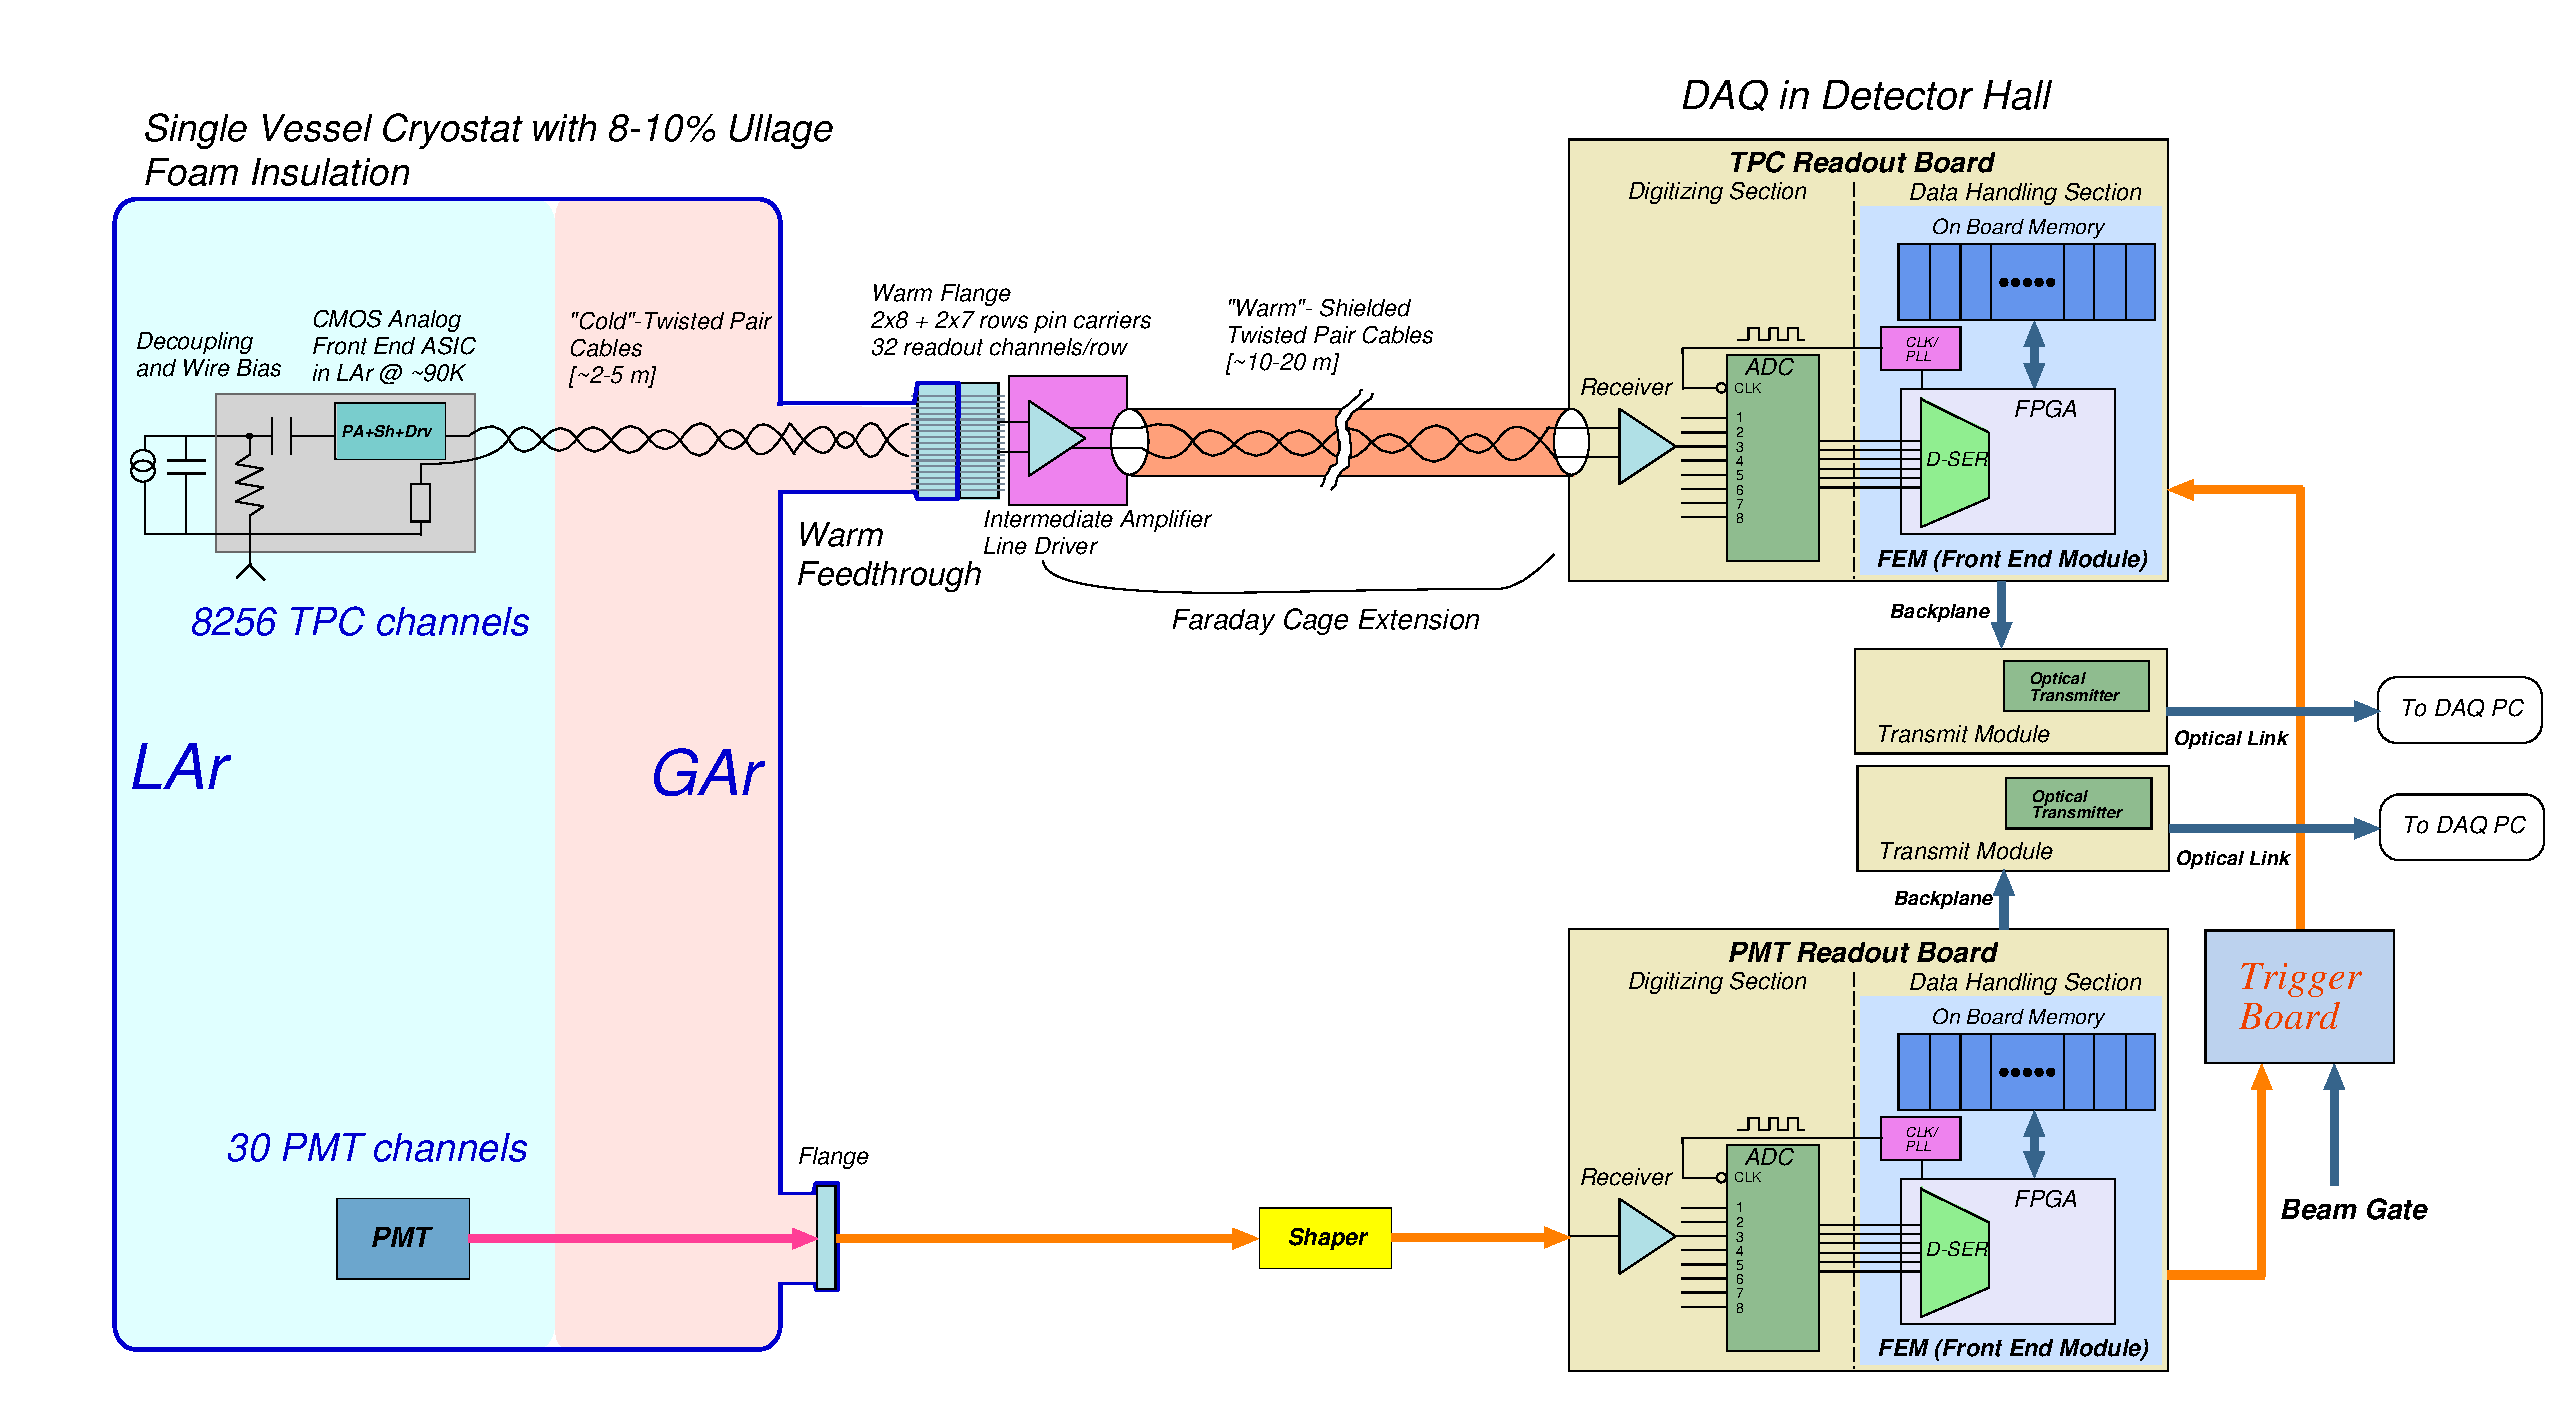
\includegraphics[width=0.9\linewidth]{./figures/MicroBooNEReadoutScheme.pdf}%
\caption{\label{readout_1}MicroBooNE \lartpc and PMT signal processing and readout stages.}
\end{figure}

%{\it{(Georgia)}}
%The MicroBooNE Readout Electronics system consists of two subsystems: the \lartpc and PMT readout electronics. The \lartpc readout electronics are responsible for the readout, digitization, and processing of the induction and collection wire signals after amplification. The PMT readout electronics are responsible for the amplification, shaping, digitization, and handling of PMT signals, as well as the trigger signal generation for the readout and data acquisition systems. While the \lartpc and PMT readout systems share the same back-end design that organizes and packages the data for delivery to the Data Acquisition (DAQ) system, they employ different analog front-end and digitization designs. 



\subsection{Cryogenic Low-Noise Electronics}
\label{sec:coldelectronics}
%{\it{(Chen)}}
To obtain optimum detector performance, MicroBooNE uses cryogenic low-noise front-end electronics for readout of the LArTPC. To reduce electronic noise, the interconnection length between the \lartpc wires and preamplifier should be as short as possible thus minimizing the total capacitance seen at the preamplifier input. To accomplish this, the analog front-end ASICs, which include a preamplifier, shaper, and signal driver are located inside the cryostat in addition to the wire bias voltage distribution system, decoupling capacitors, and calibration networks. The front-end ASIC and associated circuits are implemented on a cold mother board which is directly attached to wire carrier boards on the \lartpc itself. Cold cables are used to transmit output signals from cold motherboards to warm interface electronics installed on the top of signal feed-through flanges.

\subsubsection{CMOS ASIC}

The analog front end ASIC is designed in 180~nm CMOS technology, which integrates both the preamplifier and shaper on a single chip. Each chip has 16 channels to read out signals from 16 wires. Each channel also has a charge injection capacitor for precision calibration. In MicroBooNE, the shaper has 4 programmable gain settings (4.7, 7.8, 14 and 25 mV/fC) and 4 programmable peaking time settings (0.5, 1.0, 2.0 and 3.0 $\mu$s) that provide increased flexibility to the readout system. The ASIC also has programmable baseline settings (200 or 900 mV) to accommodate different detection wire configurations: either collection or induction plane. It has a selectable AC/DC coupling mode with a 100 $\mu$s time constant for the AC coupling mode which can be used to reduce low frequency noise. The ASIC also has built-in band-gap reference and temperature sensors to facilitate biasing and monitoring.

The CMOS ASICs consume only $\sim$6mW/channel in its default configuration. The front end ASICs of the entire detector generate $\sim$50 W of heat load that is easily handled by the cryogenics system. Design guidelines that constrain the electric field and the current density to address the lifetime of CMOS devices operated at cryogenic temperatures have been applied to every single transistor (total $\sim$15,000 transistors) in the ASIC design. A picture of the layout of the CMOS ASIC is shown in figure~\ref{fig:figasic}. Test results agree well with simulations and indicate that the analog and the digital circuits (including the digital interface) operate as expected in the cryogenic environment. 

\begin{figure}[hbt]
\centering
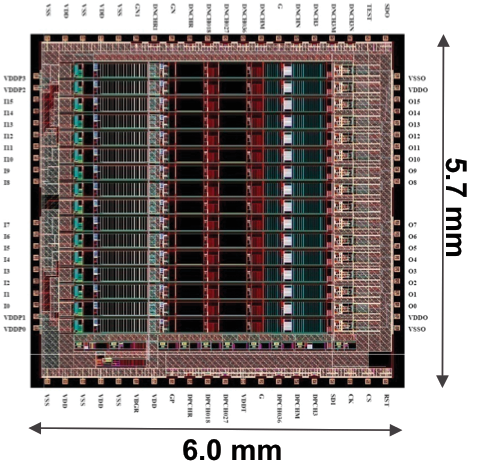
\includegraphics[width=0.75\linewidth]{figures/asic.pdf}
\caption{\label{fig:figasic}Layout of the CMOS analog front end ASIC}
\end{figure}


The MicroBooNE \lartpc has  8,256 readout channels and a total of 516 CMOS ASICs are required to fully instrument the detector. The production testing of the CMOS ASICs required two steps: both a warm and cold test. The warm test was performed with a dedicated test board housed in a Faraday box containing a socket to house the ASIC for ease in chip exchange. All programmable parameters (gain, peaking time, baseline, AC/DC coupling etc.) were exercised with the warm test setup for careful screening at room temperature. The yield of the warm testing of the ASICs was $\sim$89\%. ASICs must have passed the warm test before going through cold testing. The cold test was performed with a dedicated test board containing 6 sockets to facilitate testing of multiple chips in liquid nitrogen at the same time. A total of 201 ASICs went through cold testing with a yield of $\sim$97\%. Based on this high yield, it was decided not to continue the cold screening test on the rest of the production chips, as they were tested cold after being installed on the motherboard. After enough ($\sim$600) ASICs passed the production screening test, they were sent to an assembly house to equip the cold motherboard.



\subsubsection{Cold Motherboards}

A cold motherboard was designed to house the MicroBooNE CMOS ASICs. In this capacity, the motherboard provides signal interconnections both between the detector wires and preamplifier inputs as well as between the driver outputs and cold cables to the signal feed-through. The cold motherboard design provides sufficient protection of the ASICs against electrostatic discharge during installation. It also provides a calibration network and bias voltage distribution for the wire planes. Specifically, a calibration signal enters the cryostat via a feed-through and reaches the preamplifiers through the motherboard. Each preamplifier channel in the ASIC has a built-in switch to individually cycle the calibration injection. The bias voltage reaches the \lartpc wires via a two-fold redundant path on the motherboard that allows the detector to operate normally even if one bias voltage channel fails. Use of Rogers 4000 series as the base material of the cold motherboard avoids the potential risk of contamination of the liquid argon. The Rogers material has a similar temperature expansion coefficient as the surface mounted components which enhances the reliability of the electronics assembly when operated at cryogenic temperatures. The different positions of the wire attachments along the top and sides of the \lartpc requires 2 types of cold motherboard. The top version of the motherboard has 192 readout channels that includes 96 Y channels, 48 U channels, and 48 V channels. The side version of the motherboard has 96 readout channels that are either U or V channels. A picture of the top version of a cold motherboard with 12 mounted ASIC chips is shown in figure~\ref{fig:figmb}. 

\begin{figure}[hbt]
\centering
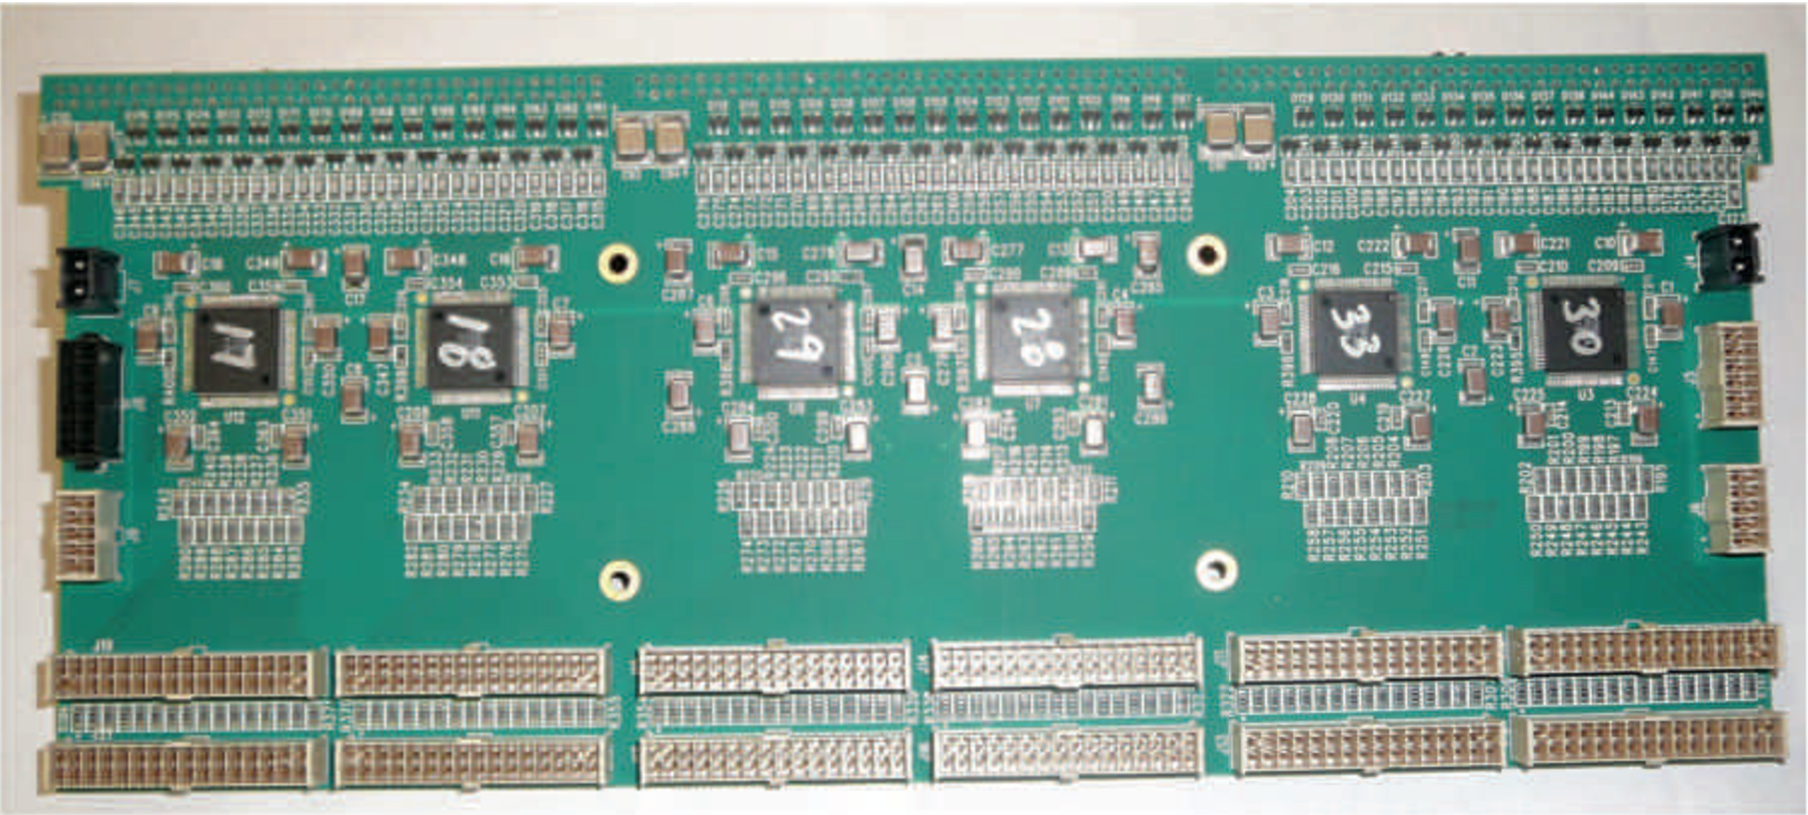
\includegraphics[width=0.75\linewidth]{figures/mb2.pdf}
\caption{\label{fig:figmb} Top version of cold motherboard with 12 ASIC chips including 6 chips are mounted on top layer and 6 chips on bottom layer}
\end{figure}


The MicroBooNE \lartpc required a total of 36 top version motherboards and 14 side version motherboards to instrument the full detector. A test stand was built for testing of the front end electronics. This test stand included a full readout chain from the cold motherboard, cold cable, signal feed-through, warm interface electronics, warm cable and Receiver ADC board to a DAQ board based on a Xilinx ML605 FPGA evaluation board which sends acquired data to a PC over a Gigabit Ethernet. The production test of each motherboard also involved both a warm and cold test. Both tests used the same test stand, except the motherboard was placed in a Faraday box for the warm test and submerged in a liquid nitrogen dewar for the cold test. Noise, gain, peaking time, and linearity parameters were measured in both warm and cold to screen the motherboard. Motherboards had to pass both tests  before being installed on the detector.

\subsubsection{Cold Cables}

Cold cables transmit the detector signals from the cold motherboard to an intermediate amplifier on top of the signal feed-through and distribute power to the CMOS ASICs. The cold cable is a custom-built 32-pair twisted pair flat ribbon cable with Teflon FEP insulation and 100$\Omega~(\pm10\%)$ impedance, using AWG 26 stranded wire with silver-plated copper. Custom designed shells with jack screws used in the cable assembly ensured proper alignment of the insertion on the signal feed-through pin carriers. The twisted pair cable was ordered from the manufacturer and sent to a company to be woven into flat ribbon cables.  Cold cables of two different formats were assembled by an assembly house: signal cables and service cables. Signal cables are used to transmit amplified detector signals while the service cable is used to transmit calibration pulses and slow control/monitoring signals. Signal cables were produced in three different lengths: 80 inch, 100 inch and 180 inch to accommodate the different lengths between the cold motherboards and the signal feedthroughs, while the service cables were produced in two different lengths: 100 inch and 180 inch. All of the cold cable assemblies were tested with a cable tester in the assembly house before they were shipped out. In addition, $\sim$10\% of the cold cables were tested in the test stand at BNL to confirm the quality of the cable assembly. 

\subsubsection{Electronic Calibration}

The MicroBooNE cold electronics include a precision charge calibration system. Through the cold cable and calibration network on the motherboard, a calibration signal enters the cryostat via a feed-through and reaches the preamplifiers. A built-in switch in the ASIC makes it possible to power cycle the calibration injection for every channel individually. The electronics calibration is based on charge injection through known capacitances (180 fF) in the ASIC. This system enables gain (charge sensitivity) calibration, verification of sense wire integrity and noise measurements. The built-in electronics calibration capability is an important tool in testing and characterizing the overall performance of the detector readout system. It was extensively used in the cold electronics production testing and the electronics checkout during installation, commissioning, and data taking.
 
\subsubsection{Performance Tests}

The development of the analog front end ASICs was initiated using 180~nm CMOS technology and 300 K models, though the performance parameters are extracted at 77 K. CMOS was found to function at cryogenic temperatures with increased gain and lower noise. The noise, gain, and pulse shaping were found to be as expected in evaluation tests of the ASICs. Extensive testing of the ASICs mounted on the motherboards was performed; these tests were done in liquid nitrogen rather than at room temperature, since noise levels and characteristics of the ASIC performance in liquid nitrogen are similar to the performance in liquid argon.  Thus, cold tests were performed on all production cold motherboards fully populated with 12 chips. A total of $\sim$2,200 chip-immersions were accumulated in liquid nitrogen without any failures due to thermal contraction or expansion. 
%($g_{m}/I_{ds}$)

\begin{figure}[hbt]
\begin{center}
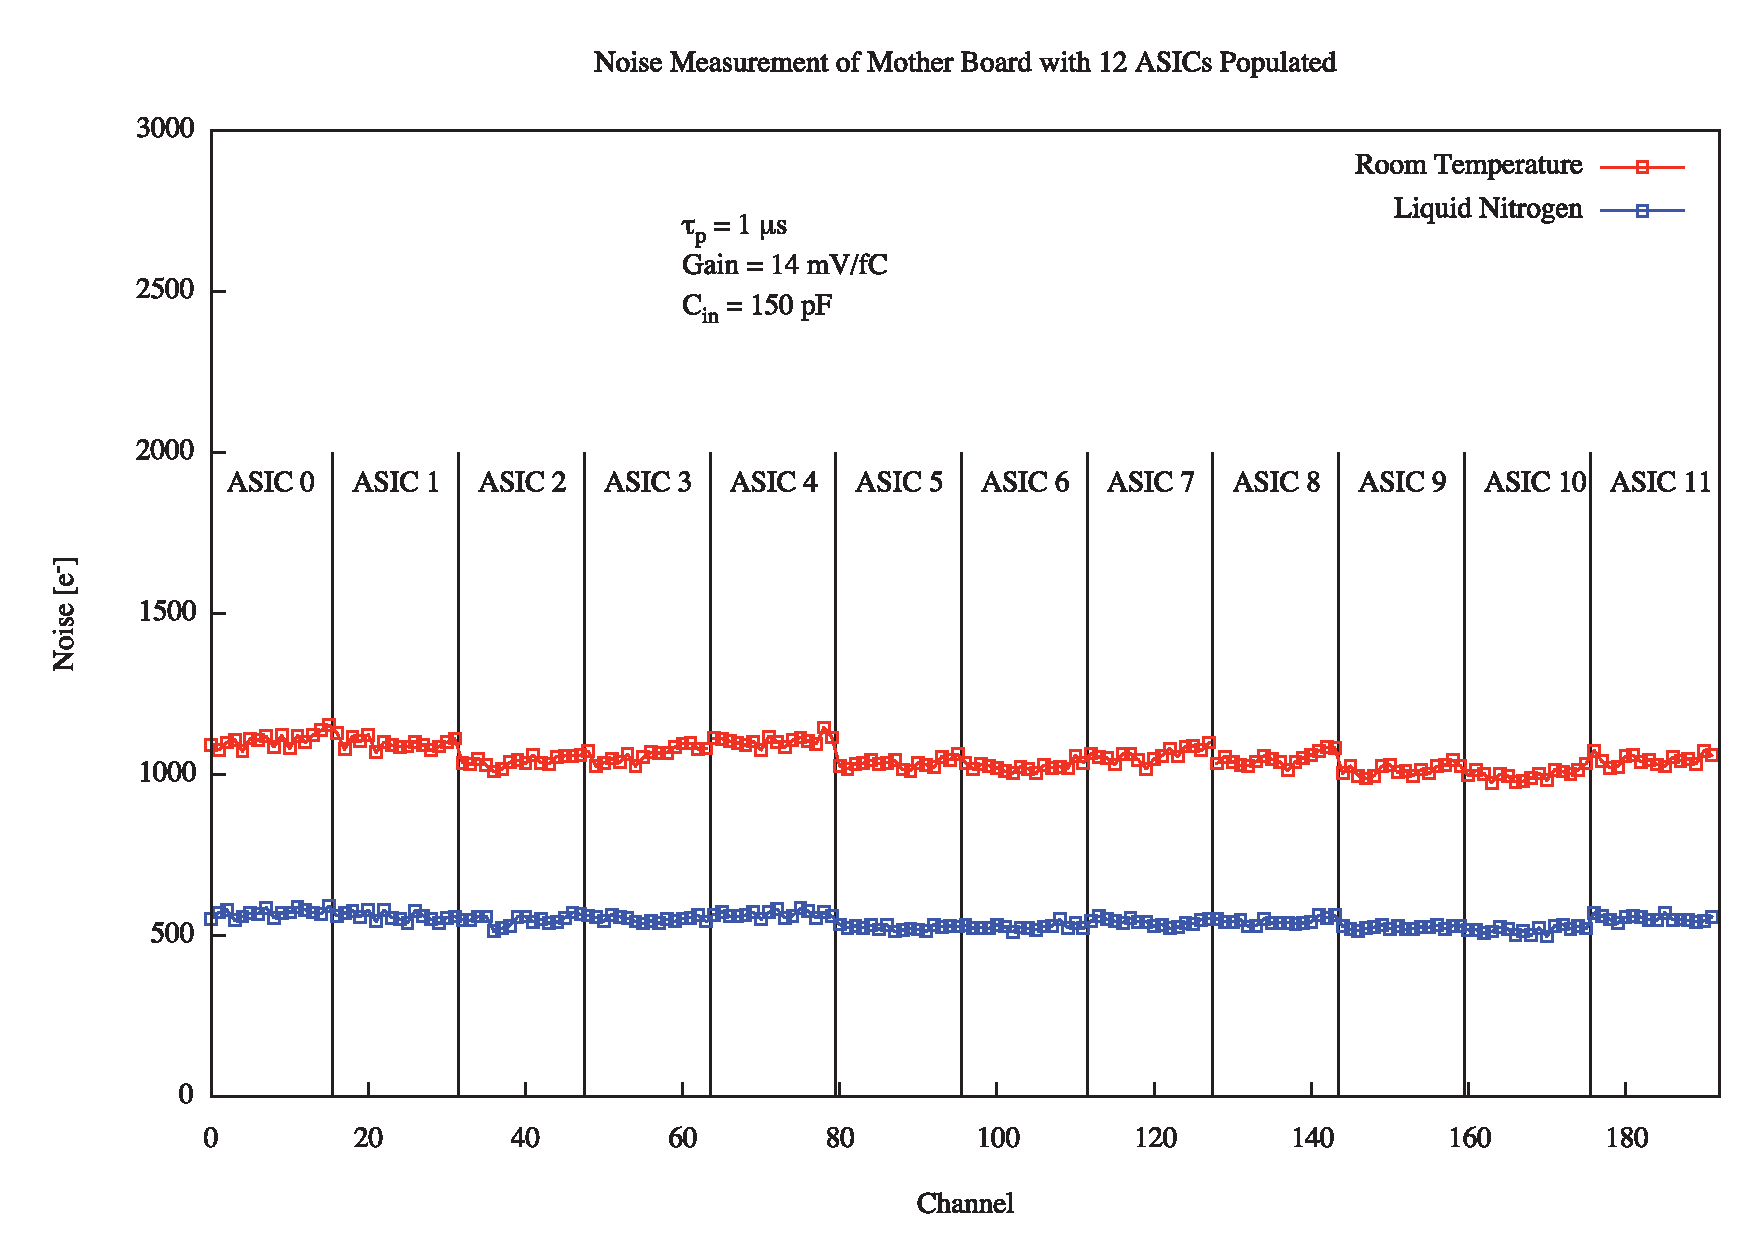
\includegraphics[scale=0.4]{figures/noise.pdf}
\end{center}
\caption{\label{fig:fignoise}Plot of noise vs. temperature of 12 ASICs, total 192 channels. Noise is $\sim$1,200$e^{-}$ at 293K, and $\sim$550$e^{-}$ at 77 K with 150 pF $C_{d}$}
\end{figure}

\begin{figure}[hbt]
\begin{center}
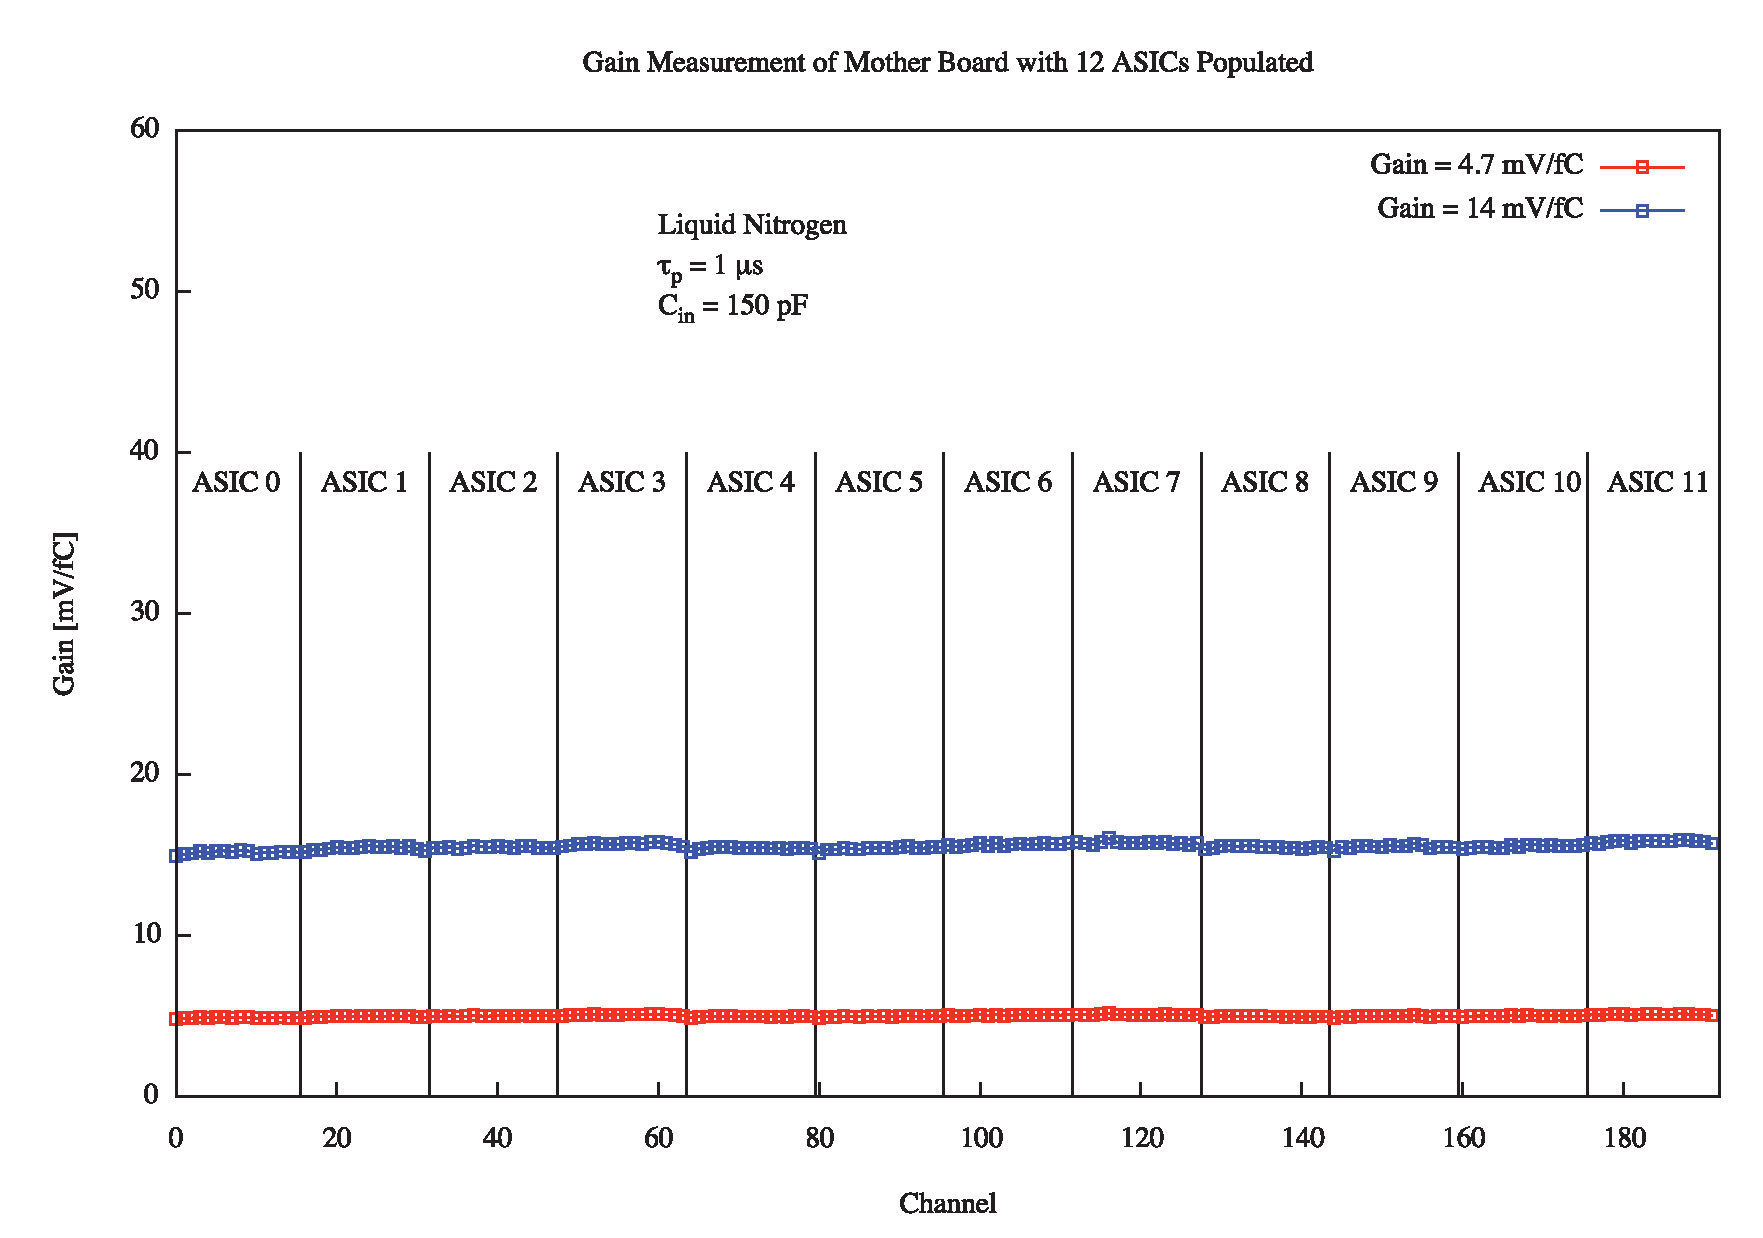
\includegraphics[scale=0.4]{figures/gain.pdf}
\end{center}
\caption{\label{fig:figgain}Plot of gain uniformity of 12 ASICs, total 192 channels, at 77~K with two different gain settings}
\end{figure}

The test results show the noise of the front end readout electronics system decreasing uniformly for all 768 channels from $\sim$1,200$e^{-}$ at 293 K to less than 600$e^{-}$ at 77 K with 150 pF detector (sense wire) capacitance. A plot of noise versus temperature of 12 ASICs for a total of 192 channels is shown in figure~\ref{fig:fignoise}. The response of the front end electronics exhibits excellent uniformity at cryogenic temperatures. As shown in figure~\ref{fig:figgain}, the gain variation of a cold motherboard with 12 ASICs is only $\sim$7\% peak-to-peak across 192 channels. The spread of the gain variation is only $\sim$1\% of the gain setting.

\subsection{Warm Electronic Amplification}
\label{sec:warmelectronics}
Signals from the cold electronics are carried over the cold cables to dedicated feedthroughs mounted on the cryostat.  The cold cables are connected to pin-carriers located on 14-inch CF signal feedthrough flanges that are mounted on nozzles N1A-N1K of the cryostat (see figure \ref{fig:cryostat-drawing}).  The signal feedthrough design must accommodate 100$\%$ hermeticity and high signal density. A design based on the ATLAS pin carrier style was developed for this purpose.  Two 8-row pin carriers and two 7-row pin carriers are welded onto the 14-inch CF flange, as shown in figure \ref{fig:feedthroughflange}, and create a vacuum-tight seal.  Nine of the 11 signal feedthroughs receive signals from the three \lartpc anode planes (384 Y-plane, 192 U-plane, 192 V-plane), while the remaining two on the extreme ends of the cryostat only receive signals from one of the angled induction planes (672 U-plane on one feedthrough, 672 V-plane on the other).

\begin{figure}[hbt]
\begin{center}
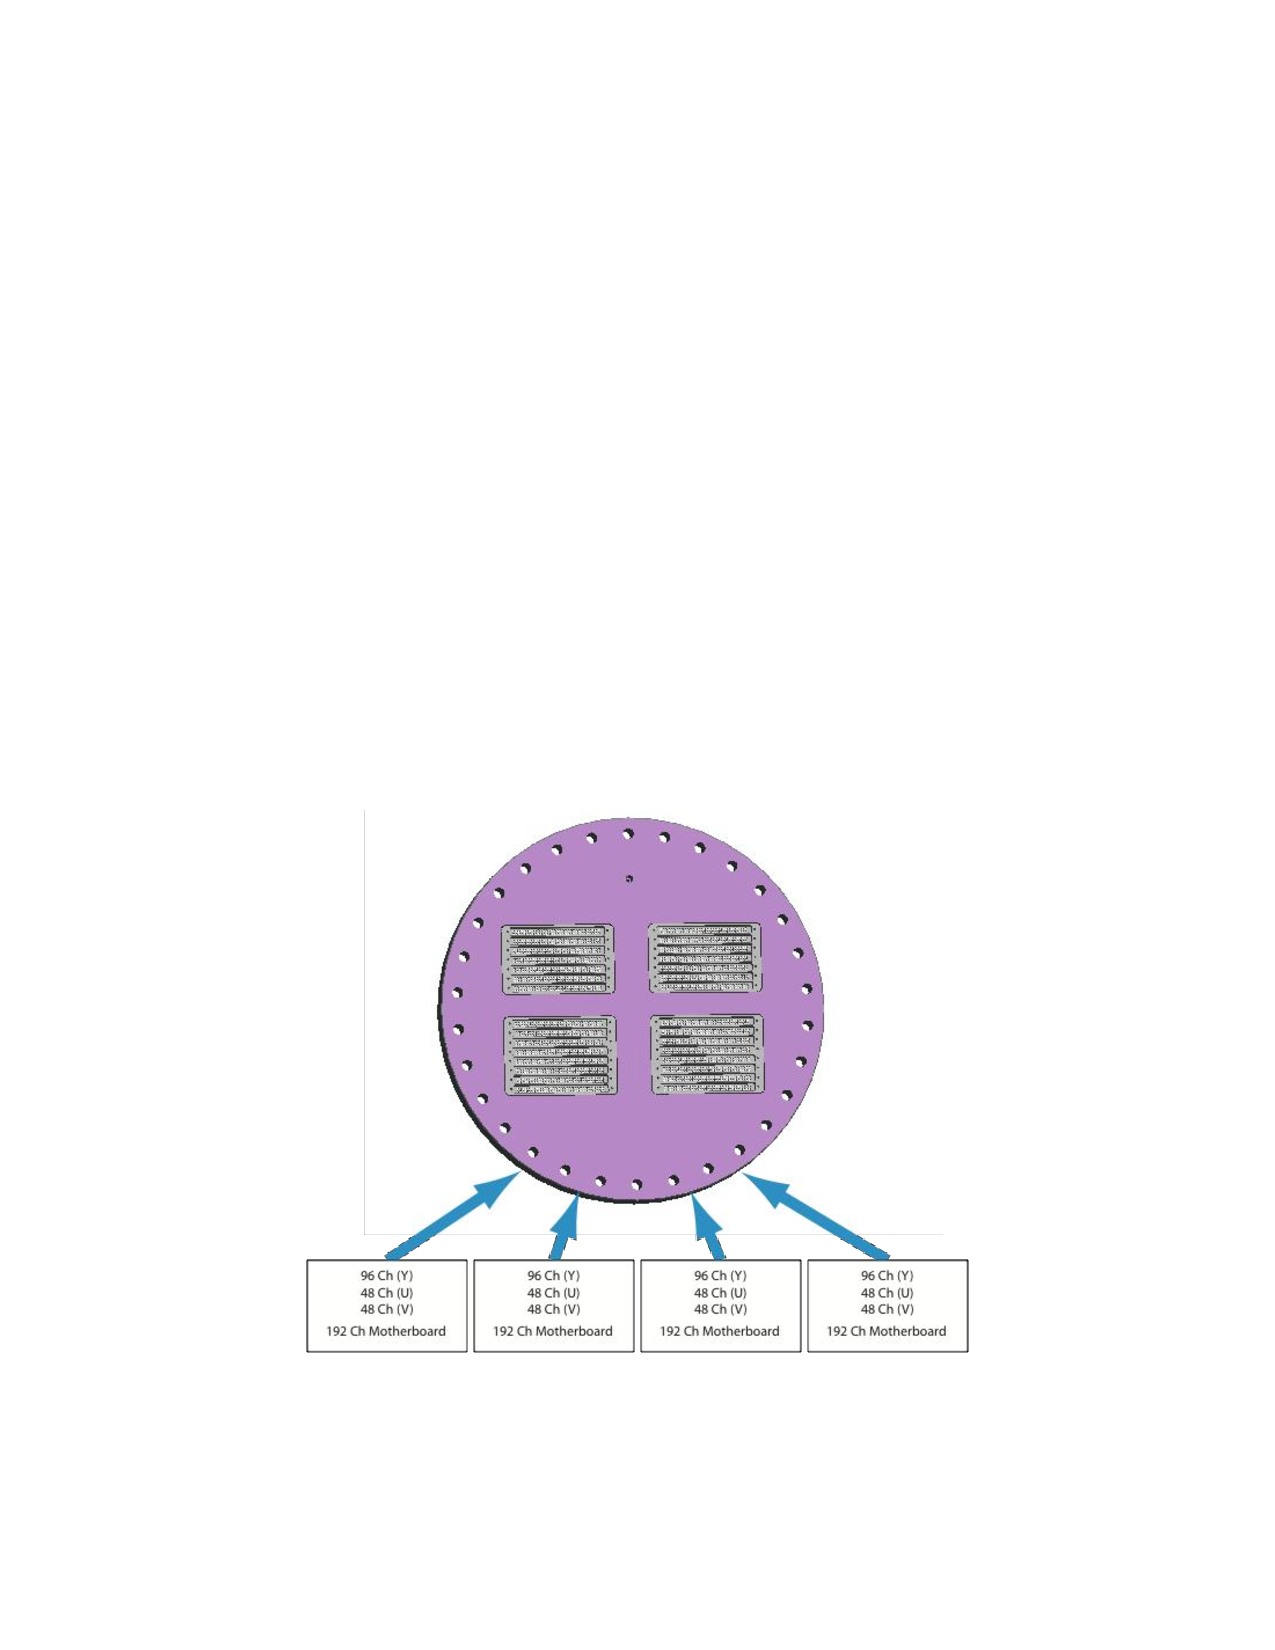
\includegraphics[width=0.8\linewidth]{figures/signal_feedthrough_standard.pdf}
\end{center}
\caption{\label{fig:feedthroughflange}Signal feedthrough flange consisting of a 14-inch CF flange with two 8-row and two 7-row pin carriers welded in place.}
\end{figure}

A Faraday cage is mounted on the external, warm, side of the signal feedthroughs to provide shielding for the intermediate amplifiers located inside.  The bias voltage feedthrough, which supplies anode plane bias voltages into the cryostat, is built onto a small 2.75-inch CF flange welded onto the signal feedthrough flange. A filter board mounted on the bias voltage flange filters noise and ensures a good ground connection. Figure \ref{fig:feedthroughassembly} shows details of the signal feedthrough assembly with electronics boards, bias voltage feedthrough, and Faraday cage.

\begin{figure}[hbt]
\begin{center}
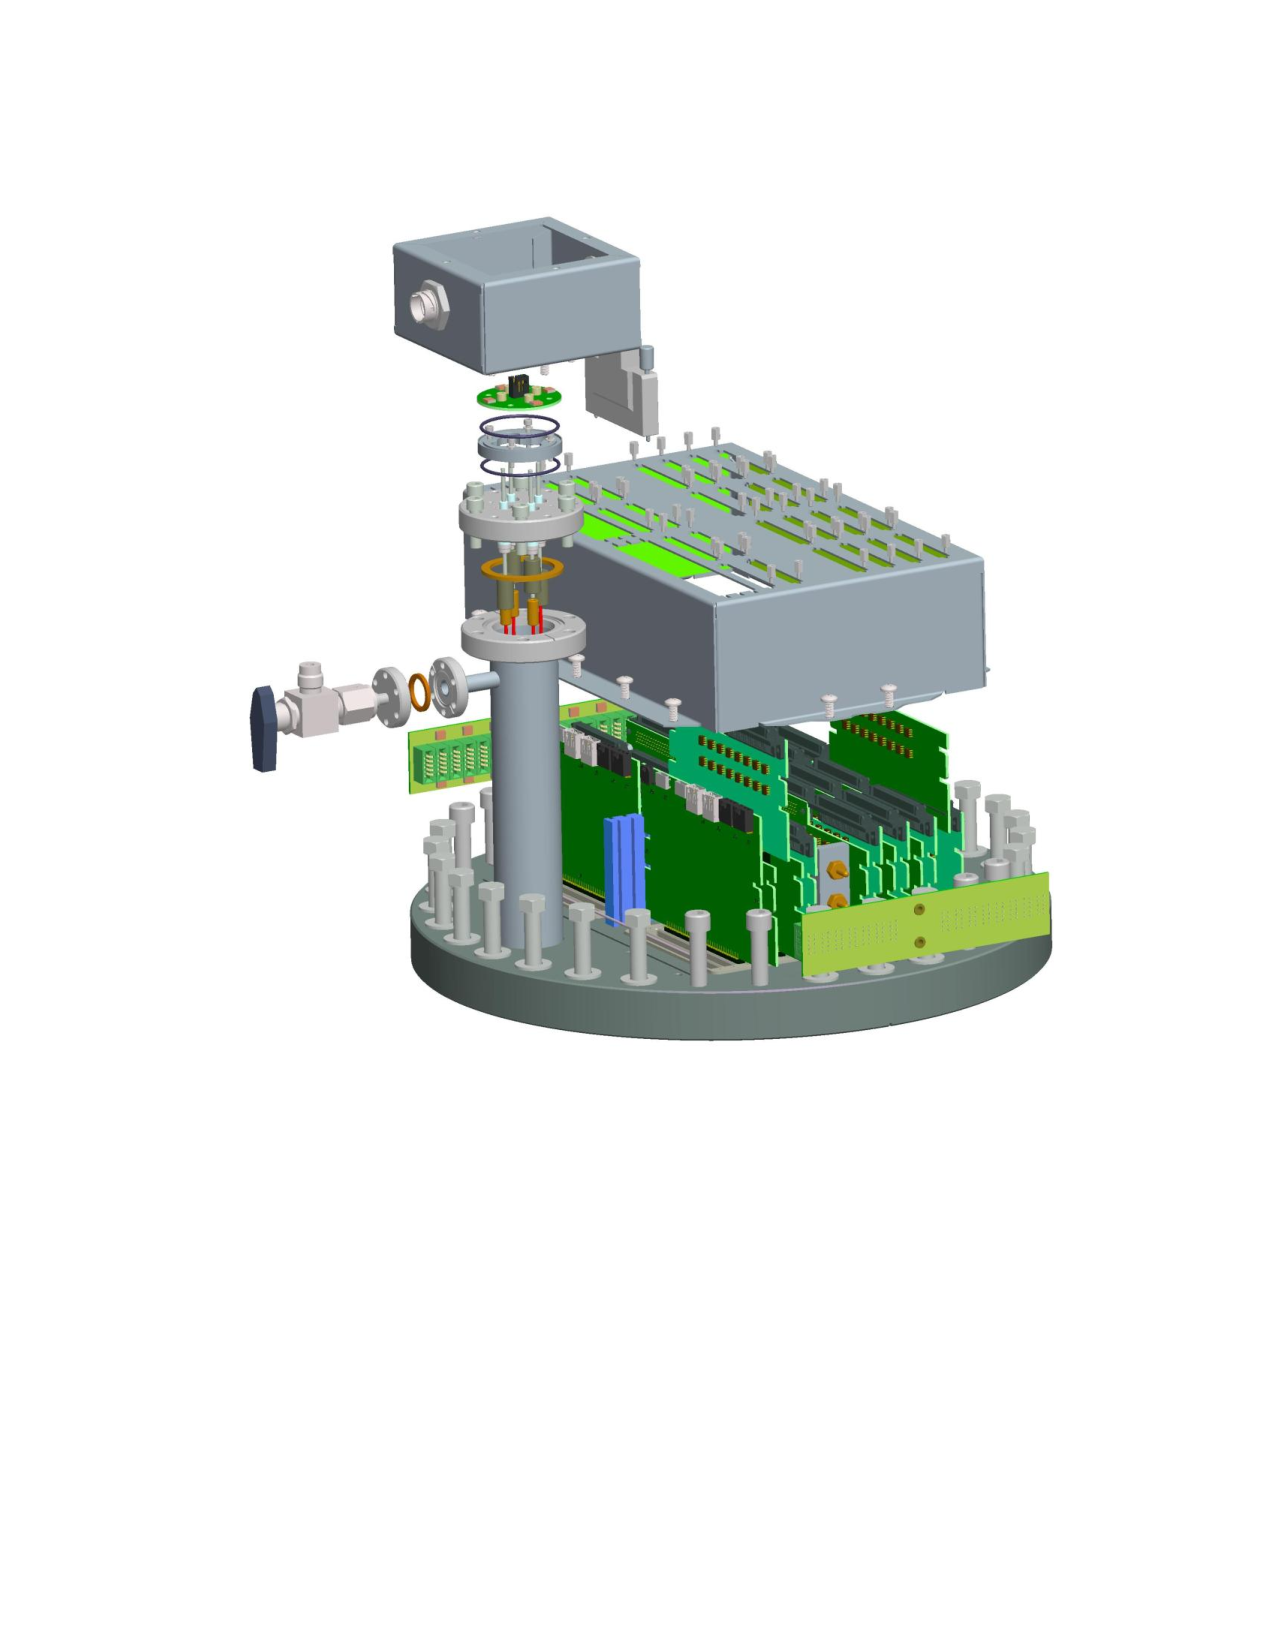
\includegraphics[width=0.4\linewidth]{figures/signal_feedthrough_assembly.pdf}
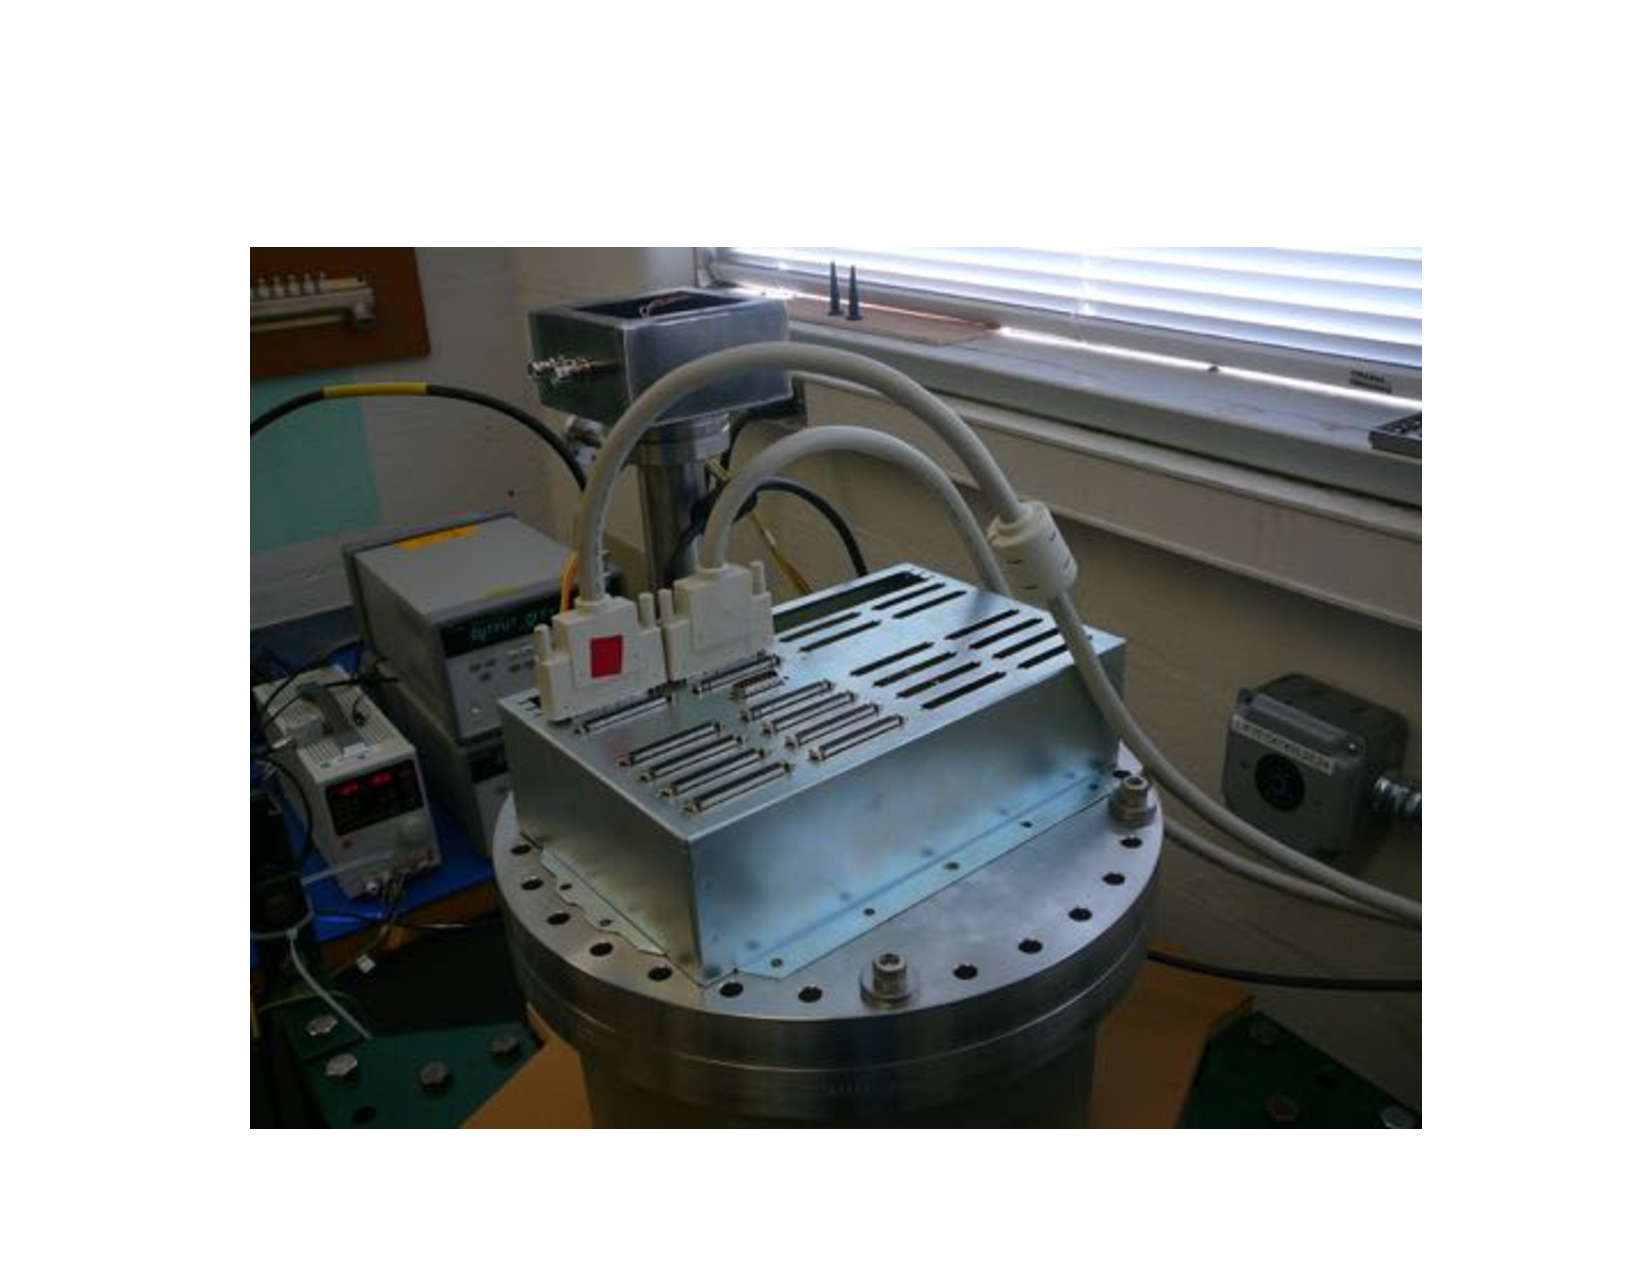
\includegraphics[width=0.4\linewidth]{figures/signal_feedthrough_assembly_photo.pdf}
\end{center}
\caption{\label{fig:feedthroughassembly}Left:  Diagram of the signal feedthrough assembly, which includes intermediate amplifiers, Faraday cage, bias-voltage feedthrough and filtering circuit.  Right: Photograph of one of the feedthrough assembly, partially constructed and being tested.}
\end{figure}

The intermediate amplifiers provide $\sim$12 dB gain to the \lartpc signals to make them suitable for transmission over a 20 m long cable to the readout electronics (see section \ref{sec:readoutelectronics}).  Each intermediate amplifier has 32 channels installed on the signal feedthrough flange and housed inside the Faraday cage to provide noise isolation. Figure \ref{fig:intermediateamplifier} shows a picture of a prototype intermediate amplifier plugged on the signal feedthrough pin carrier. The intermediate amplifier uses a 68-pin SCSI-3 connector to drive the 32 channels of signal differentially for better noise immunity. The layout and connector position have been carefully designed to ensure the card can be plugged on the pin carrier in either direction. This efficiently utilizes the limited available space on the top of the feedthrough, which also makes the design of the Faraday cage easier.

In addition to the intermediate amplifiers, there are two service boards mounted on the top of each signal feedthrough. The service board provides regulated low voltage, control and monitoring signals to the analog front end ASICs. It also provides pulse injection to the preamplifiers for precision calibration. The control, monitoring, and calibration signals are provided to the front end electronics with two-fold redundancy. Should one set of signals become defective the detector can still operate normally with the redundant set. Each service board plugs onto a 64-pin carrier row. Figure \ref{fig:intermediateamplifier} shows a picture of a prototype service board.

\begin{figure}[hbt]
\begin{center}
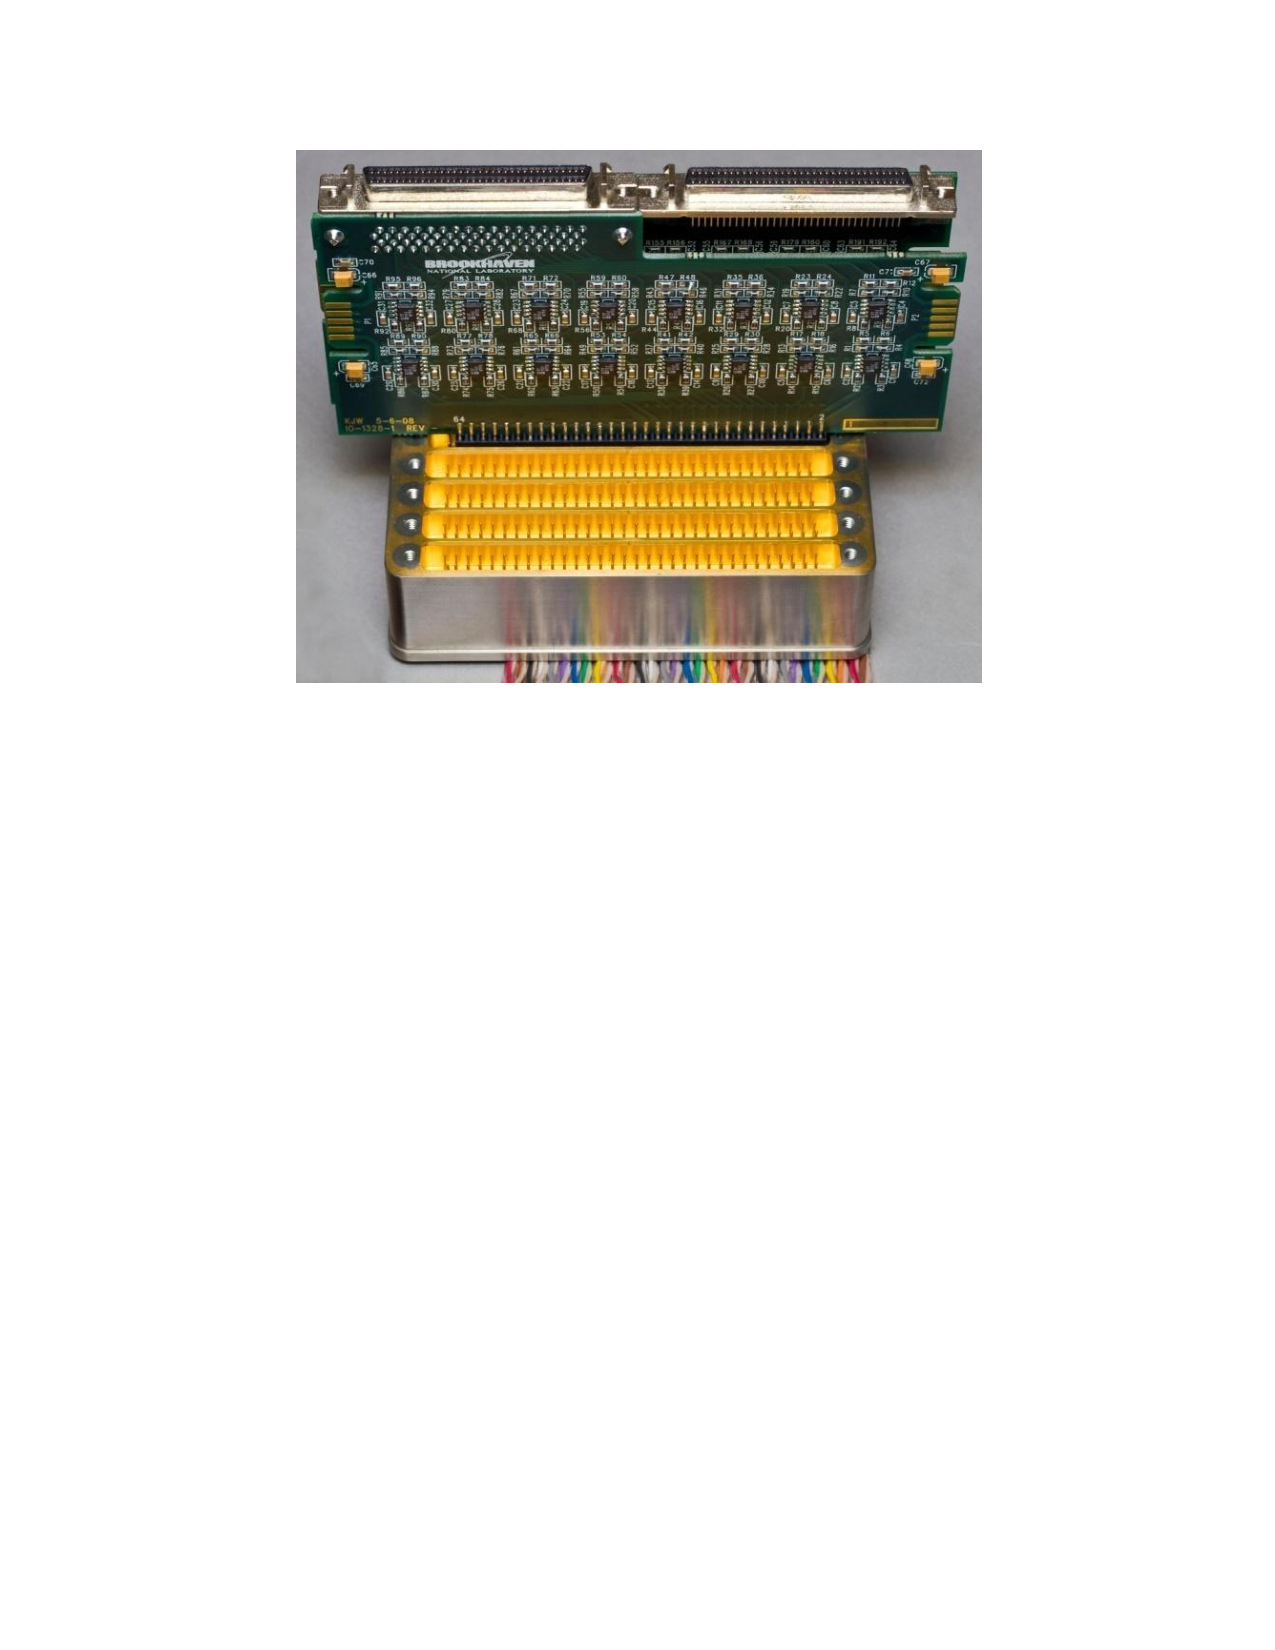
\includegraphics[width=0.4\linewidth]{figures/intermediate_amplifier.pdf}
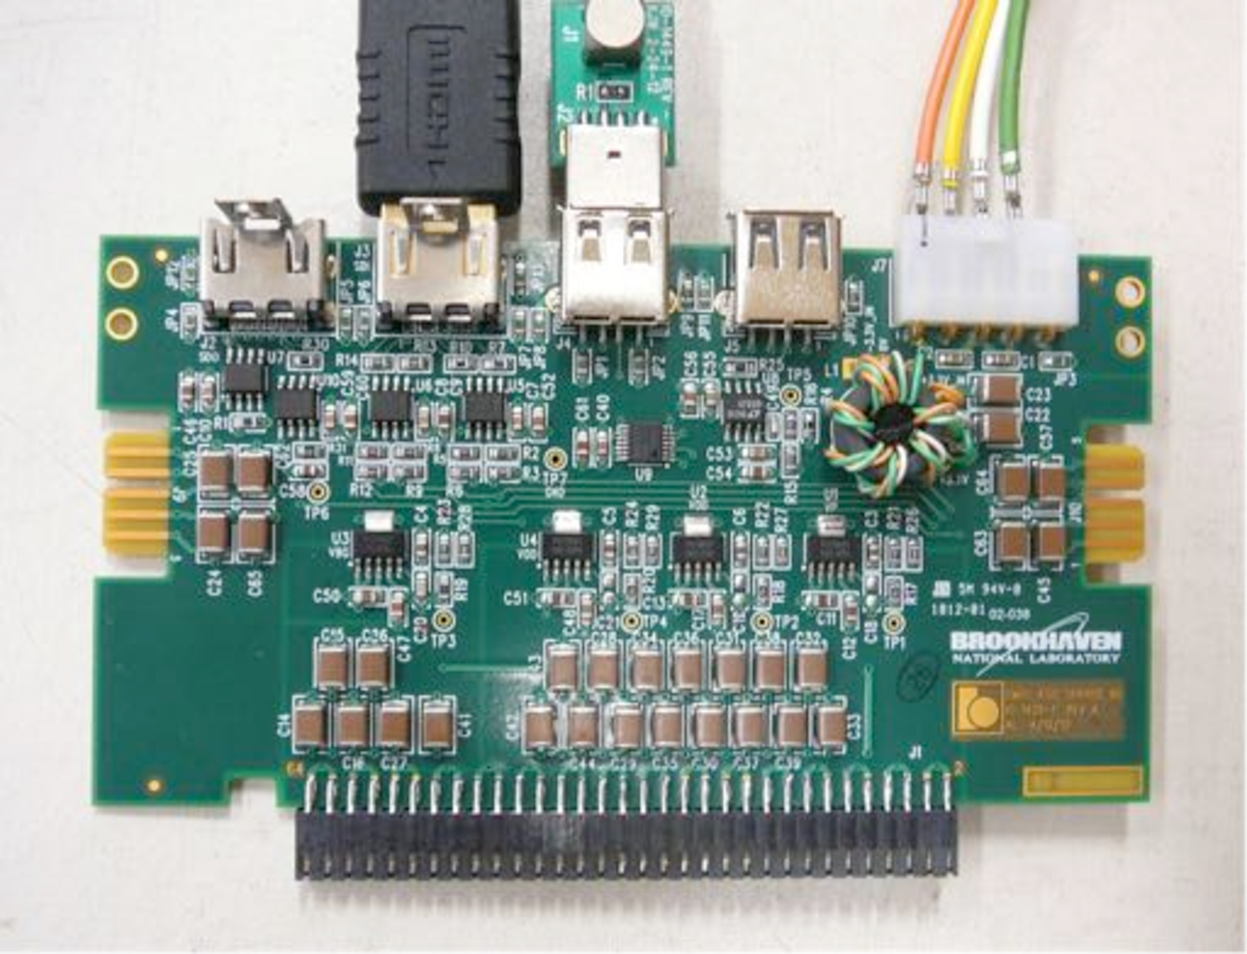
\includegraphics[width=0.4\linewidth]{figures/serviceboard.pdf}
\end{center}
\caption{\label{fig:intermediateamplifier}Left: Photograph of one of the intermediate amplifier boards plugged into a pin carrier during testing.  Right: Photograph of a prototype service board.}
\end{figure}


\subsection{Readout Electronics}
\label{sec:readoutelectronics}
%{\it{(Georgia)}}
The MicroBooNE readout electronics system consists of two subsystems: the \lartpc and PMT readout electronics. The \lartpc readout electronics are responsible for the readout, digitization, and processing of the induction and collection wire signals after amplification. The PMT readout electronics are responsible for the amplification, shaping, digitization, and handling of PMT signals, as can be used to provide a trigger signal for the readout and data acquisition systems. While the \lartpc and PMT readout systems share the same back-end design that organizes and packages the data for delivery to the DAQ system, they employ different analog front-end and digitization designs, which are described in this and the following subsection.

The \lartpc readout electronics are responsible for processing the signals from the 8,256 wires in MicroBooNE after pre-amplification and shaping in the cold electronics (section~\ref{sec:coldelectronics}).  The pre-amplified and shaped analog signals from the cold electronics are transmitted to the warm electronics outside the cryostat, as described in section~\ref{sec:warmelectronics}, and then passed to custom-designed \lartpc readout modules distributed evenly over nine readout crates.  The readout modules digitize the analog signals and then process and prepare them for shipping to designated DAQ machines (one per readout crate) (section~\ref{sec:daq}). 

The \lartpc readout crates communicate with the DAQ machines via three duplex 3.125 Gbits/sec optical links that connect to a crate controller module and data transmitter (XMIT) module on the crate end, and to three PCI Express boards on the DAQ machine end. The controller is responsible for configuration, trigger and run control command distribution as well as the slow monitoring of each readout crate. The controller occupies one of the optical links while the XMIT is responsible for sending two separate streams of readout data to the DAQ machines via the two other optical links. The first XMIT stream contains losslessly compressed \lartpc data associated with event triggers received by the \lartpc readout crates, such as the BNB trigger, and is referred to as the ``NU'' data stream. The second stream is a continuous \lartpc data stream which is compressed with some data loss. The continuous data stream is used for beam-unrelated physics analyses, such as the study of potential supernova neutrino events, and is referred to as the ``SN'' data stream. The compression schemes used in the NU and SN streams are described in section~\ref{sec:tpccomp}.

All readout crates are synchronized to a common 16 MHz clock. The clock sync is provided by a clock fanout board which shares the same ground as all readout crates, and is sent via coaxial cable to a distribution board which is mounted on each crate backplane. The readout frame size is set to 1.6 ms, which is equivalent to the time it takes for charge produced on the far end of the \lartpc to drift to the wire planes at the design cathode voltage of -128 kV.

\subsubsection{\label{sssec:tpcdigitization} Data Digitization}

The amplified and shaped analog \lartpc signals are differentially received and digitized in the first section of the readout modules. Each ADC module holds 8 AD9222 octal-channel 12-bit ADCs. Each ADC module handles signals from 64 wires. The wire signals are grouped in two sets of 32 consecutive wire channels: either 32 induction wires plus 32 collection wires or two sets of 32 induction wires. The induction channel sequence alternates wires between the two induction planes. The ADC module digitizes the signals continuously at 16MHz. Each channel has a configurable baseline, which is either set low (450 ADC counts) for collection channels or at the middle of the dynamic range (2055 ADC counts) for induction channels, thus ensuring that both the collection plane unipolar differential signals and the induction plane bipolar differential signals can make use of the full ADC analog input range. The requirement to observe a MIP produced at the far end of the \lartpc in the induction plane determines the lower end of the dynamic range, while the requirement to observe a highly-ionizing stopping proton at the close end of the \lartpc without saturation sets the upper end. The digitized outputs from the ADC board are passed directly to a Front End Module (FEM) in the second section of the \lartpc readout module. The FEM houses an FPGA for data processing, data reduction, and preparation for readout by the DAQ system as described in the following section. 

\subsubsection{\label{sssec:tpcFEM} Data Handling}

The FEM board consists of a 14-layer printed circuit board which is mechanically integrated with the ADC board as illustrated in figure~\ref{fig:readout_2}. The choice of a smaller board allows for short trace lengths which is beneficial for high speed signals. The full assembly comes together as a standard VME 9U card in height, with a 280 mm depth. Differential outputs from the ADCs connect to the FPGA through HM-Zd connectors that have individual ground shielding on each differential pair. 

\begin{figure}
\centering
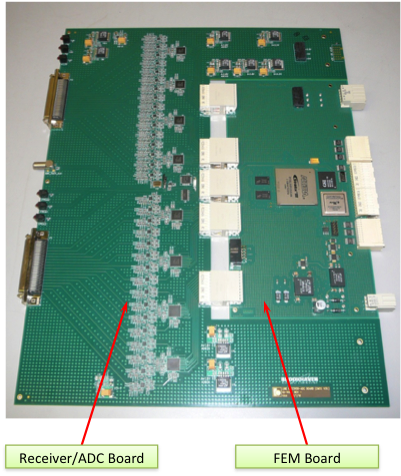
\includegraphics[width=0.6\linewidth]{./figures/readout_2.png}%
\caption{\label{fig:readout_2}\lartpc ADC+FEM board.}
\end{figure}

The digitized data stream moves from the ADCs to a Stratix III Altera FPGA, which reduces the sampling rate of the ADC from 16~MHz to 2~MHz. The 2~MHz sampling rate is optimized by taking into consideration the expected pulse shape provided by the convolution of the cold electronics, the expected \lartpc field responses, and the O(1$\mu$s) diffusion effects which govern charge drift within the liquid argon. The FPGA stores the data from all 64 wires per board sequentially in time in a 1M $\times$ 36 bit 128 MHz SRAM, grouping two ADC words together in each 36 bit memory word. This requires a data storage rate of (64/2) $\times$ 2 MHz $=$ 64 MHz.  The SRAM chip size and memory access speed allow for continuous readout of the \lartpc data. Since data reduction and compaction algorithms rely on the sequential time information of a given wire, the data readout out from this SRAM takes place in wire order in alternate clock cycles, again at the rate of 64 MHz. This read in/out sequence is illustrated in figure~\ref{fig:readout_3}.

\begin{figure}
\centering
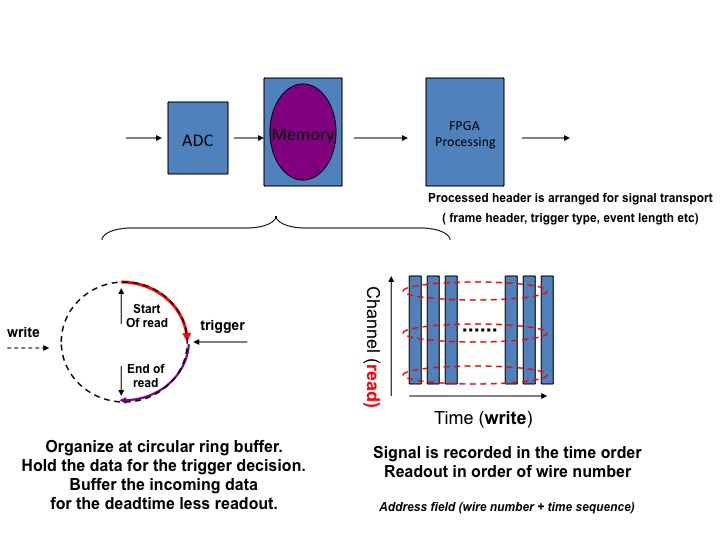
\includegraphics[width=0.8\linewidth]{./figures/readout_3.jpg}%
\caption{\label{fig:readout_3}\lartpc readout sequence in the TPC FEM.}
\end{figure}

Separate DRAM multi-event buffers on the FEM store the NU and SN data streams. The data divert into the NU readout stream when a trigger is issued and received (as shown in figure~\ref{fig:readout_4}) which signals, for example, an accelerator neutrino-induced event. When an event trigger is received, 4.8 ms worth of data, relevant to that event, are packeted per channel and sent to the DAQ through the NU data stream. The 4.8 ms readout size is governed by the maximum drift time and spans three or four frames. In order to reduce the amount of data being transmitted, the FPGA trims the three or four frames to span the exact 4.8 ms required, 1.6 ms before the trigger plus 3.2 ms after the trigger. In parallel, the data is continually sent out through the SN data stream, frame by frame. The compression and data reduction algorithms applied to each of the two streams are described in the following section.
 
\begin{figure}
\centering
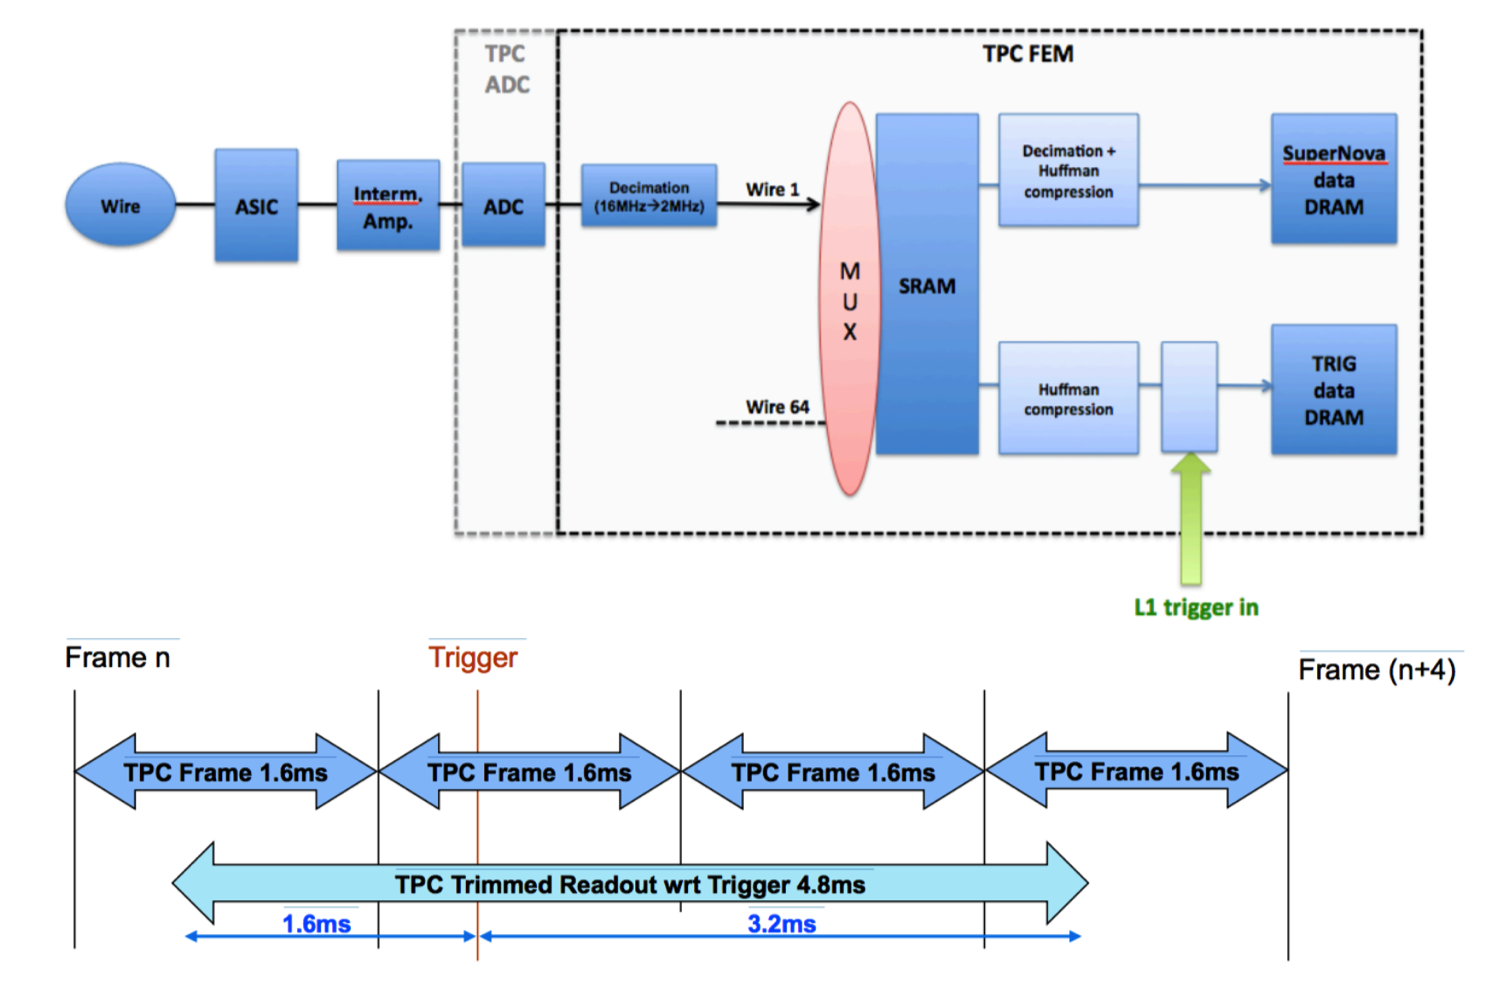
\includegraphics[width=0.8\linewidth]{./figures/readout_4.png}%
\caption{\label{fig:readout_4}\lartpc trigger readout.}
\end{figure}

After processing by the FPGA, the data passes to the crate backplane dataway on connectors shown in figure~\ref{fig:readout_2}. A token-passing scheme is utilized to transfer data from each FEM board to the data transmitter module (XMIT) in a controlled way, whereby each FEM, in the order of closest to furthest from the XMIT module, receives a token, transmits its data to the XMIT, and passes the token on to the next FEM in the sequence. For the NU stream, each FEM sends all data associated with a particular trigger number; while for the SN stream, each FEM sends all data associated with a particular frame number. This data transfer is relayed via the otherwise passive crate backplane, and is limited to 512~MB/s. In the XMIT module, the data is buffered temporarily and sent to the DAQ machine through the two streams, SN and NU, which proceed effectively in parallel.

%\begin{figure}
%\centering
%
\includegraphics[width=0.8\linewidth]{./figures/temp}%
%\caption{\label{fig:readout_5}Picture of connectors on dataway? \textbf{NOTE:  Missing Image!}.}
%\end{figure}


\subsubsection{Compression Schemes}
\label{sec:tpccomp}

In the case of the NU data stream, a lossless Huffman coding scheme implemented in the FEM FPGA compresses the data by approximately a factor of five. Further reduction in the overall rate is achieved by exploiting a PMT trigger in coincidence with the BNB trigger, as described in section~\ref{sec:trigger}. Huffman coding provides for lossless data compression by taking advantage of the slow variation of the waveform TPC data in any given channel. In particular, this compression scheme relies on the fact that successive data samples on any given wire vary relatively slowly in time. As such, when noise levels are low, any two adjacent data samples either coincide or differ by 1 ADC count. The most frequent values for the difference in ADCs between successive data samples are assigned pre-specified bit patterns with the lowest number of bits possible. Those bit patterns are encoded in the 16-bit data words that would otherwise be used for a single 12-bit ADC sample value. As such, data reduction of up to a factor of 14 is theoretically possible\footnote{The uppermost two bits are always reserved for header information, in each 16-bit word.}. In practice, the data reduction is sensitive to noise levels and \lartpc activity, and is also dependent on the gain setting. The compression factor achieved by MicroBooNE is shown in figure~\ref{fig:readout_6}.

\begin{figure}
\centering
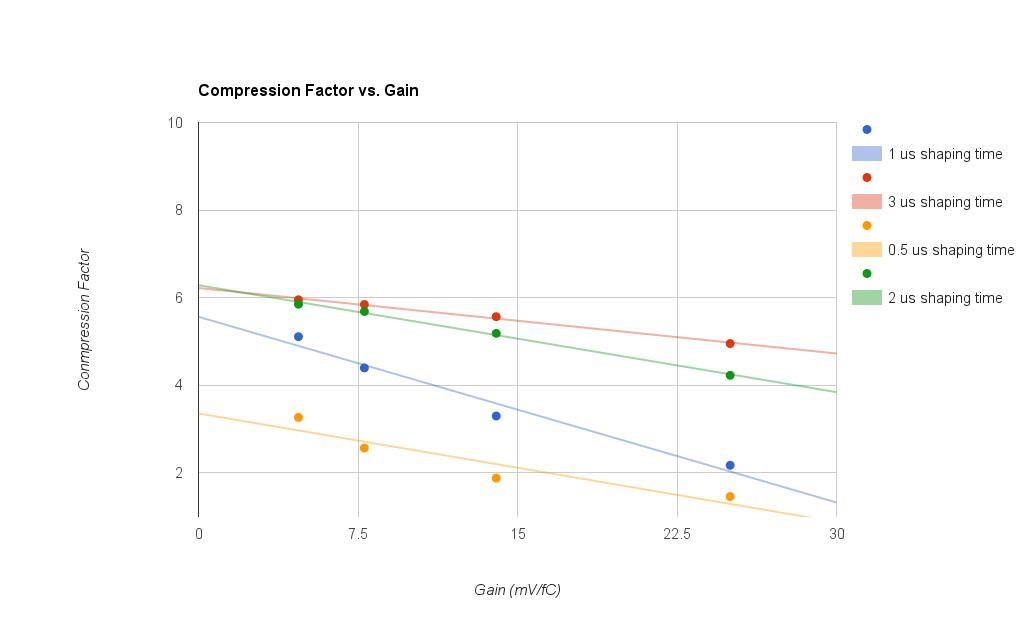
\includegraphics[width=0.8\linewidth]{./figures/readout_6.jpg}%
\caption{\label{fig:readout_6}Compression factors achieved on ADC data with Huffman compression.}
\end{figure}

Because of the low trigger rate\footnote{The BNB trigger dictates an upper bound on the trigger rate of 15 Hz.}, lossless Huffman coding compression proves sufficient for the NU data stream. However, for the continuous SN stream, further compression becomes necessary, resulting in unavoidable data loss. A method called ``dynamic decimation'' (DD) handles this case. The DD scheme relies on recognizing regions of interest (ROI) in the data stream that contain waveforms corresponding to drift ionization charges. Portions of the data stream not containing ROI contribute to pedestal determination, and ROI are identified as deviations from the continually-updated pedestal, buffered, and read out to disk. At the time of this writing, the MicroBooNE SN stream compression scheme is being finalized and the SN readout stream will be commissioned in September 2016.

\subsection{PMT Readout Electronics}

The PMT readout electronics are responsible for processing signals from the 32 PMTs described in section~\ref{sec:light-collection} and identifying light signatures coincident with the BNB and NuMI beam spills. The coincidences generate PMT triggers that can be later mixed with other triggers in the Trigger Board (TB). Signals from the 4 light paddle guides installed in the \lartpc are also recorded by the PMT readout electronics, but these signals do not participate in the PMT trigger generation. 

The stages of signal processing are illustrated in figure~\ref{fig:readout_7}. First, each PMT signal (with the exception of the light paddle guide signals) is split into two different gains, as described in section~\ref{LCUnitimplement}, with the HG channel carrying 18$\%$ of the PMT signal and the LG channel carrying 1.8$\%$ of the PMT signal. Each gain is split once again into HG1 and HG2, and LG1 and LG2, in order to allow different processing of beam-related and beam-unrelated PMT signals. All 32$\times$2$\times$2 plus 4 signals are pre-amplified and shaped in 16-channel pre-amp/shaper boards (section~\ref{sec:PMTamp}). Four PMT readout modules receive the analog shaped signals differentially and digitize them (section~\ref{sec:pmtdigit}) at 64 MHz. The PMT readout modules then process the signals in order to prepare them for shipping to a designated DAQ machine and to form a possible PMT trigger (section~\ref{tpcfem}). 

Each one of the 4 PMT ADC+FEM readout boards used in the PMT readout system handles one of the following:

\begin{itemize}
\item Readout of and PMT trigger generation using the HG1 PMT signals associated with neutrino beam events. The paddle signals are also readout by this board. 
\item Readout of and PMT trigger generation using the HG2 PMT signals that are out of beam time (i.e. cosmic rays and other cosmogenic backgrounds) 
\item Readout of the LG1 PMT signals associated with neutrino beam events
\item Readout of the LG2 PMT signals that are out of beam time
\end{itemize}

\begin{figure}
\centering
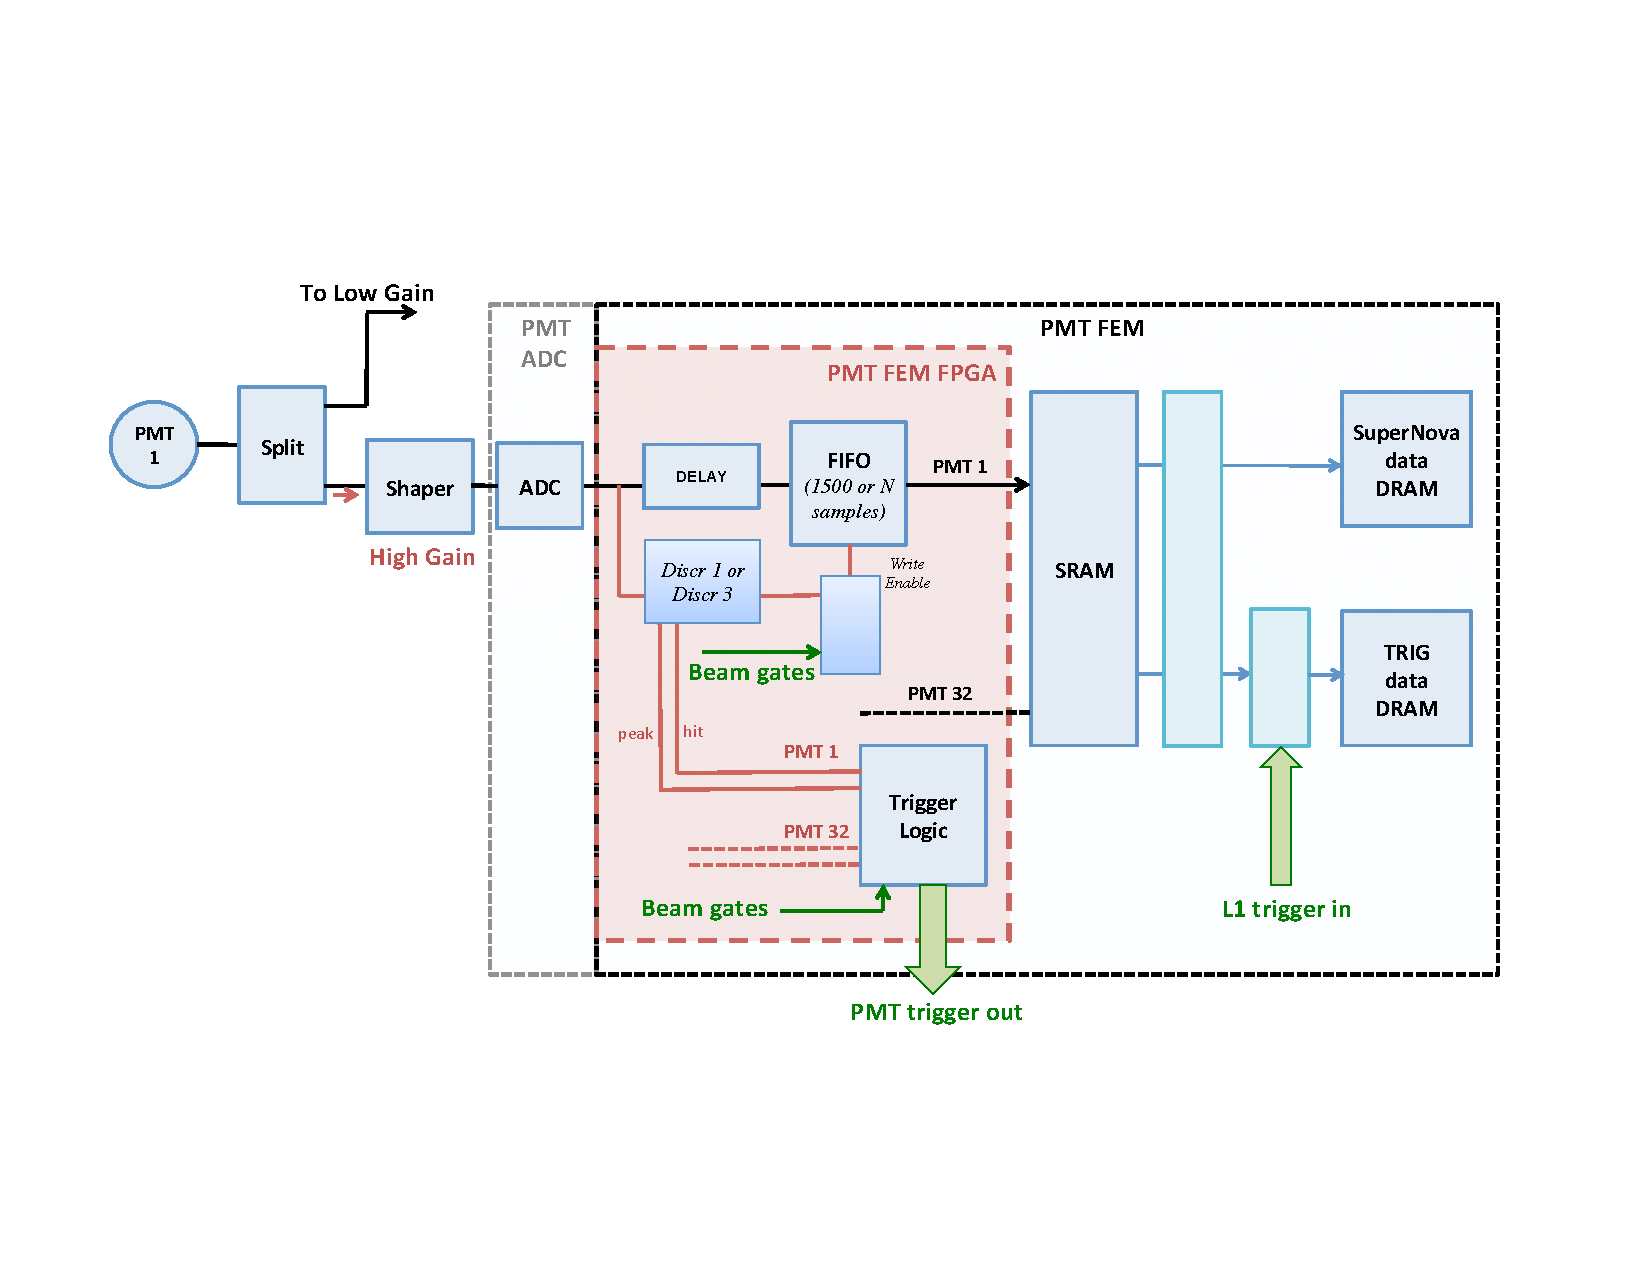
\includegraphics[width=0.8\linewidth]{./figures/readout_7}%
\caption{\label{fig:readout_7}Signal processing in PMT FEM.}
\end{figure}

After signal processing, the data is sent to a designated DAQ machine via a transmitter (XMIT) module in the same way as is done for \lartpc data. Two data streams are provided: a NU data stream associated with event triggers and a SN data stream which a continuous version of the NU stream readout.

\subsubsection{\label{sec:PMTamp}Signal Amplification and Shaping}

The preamp/shaper boards read raw PMT signals from the PMT HV/signal splitters and shape them into unipolar signals with a 60 ns rise time. The shaped signals are sent to the \lartpc readout boards differentially via short front-panel cables, in order to minimize noise, where they are digitized at 64 MHz. The 60 ns peaking time allows digitization of two or three samples on the rising edge. This in turn enables an accurate determination of the event start time ($t_0$) needed to determine the $x$ coordinates of ionization signals along the drift direction. An accurate time measurement also helps reject other tracks, such as cosmic rays, that cross the detector during the drift time.

\subsubsection{PMT Data Digitization}
\label{sec:pmtdigit}

The ADC (Texas Instruments, ADS5272) module part of the PMT readout board (figure~\ref{fig:readout_8}) is responsible for digitization of up to 48 differentially-driven input signals. The differential signals are digitized at 64~MHz. The 64 MHz clock used by the PMT readout is generated starting from the 16 MHz clock that is common to all readout crates (\lartpc and PMT). 

%, subtracted, and discriminated using a two-level discriminator scheme. A low discriminator, $d_0$, is used to provide a good timing resolution, while a second, higher discriminator which is active only after the $d_0$ discriminator has been met, is responsible for pushing a pre-configurable number of consecutive ADC pulses to a FIFO buffer. 

\begin{figure}
\centering
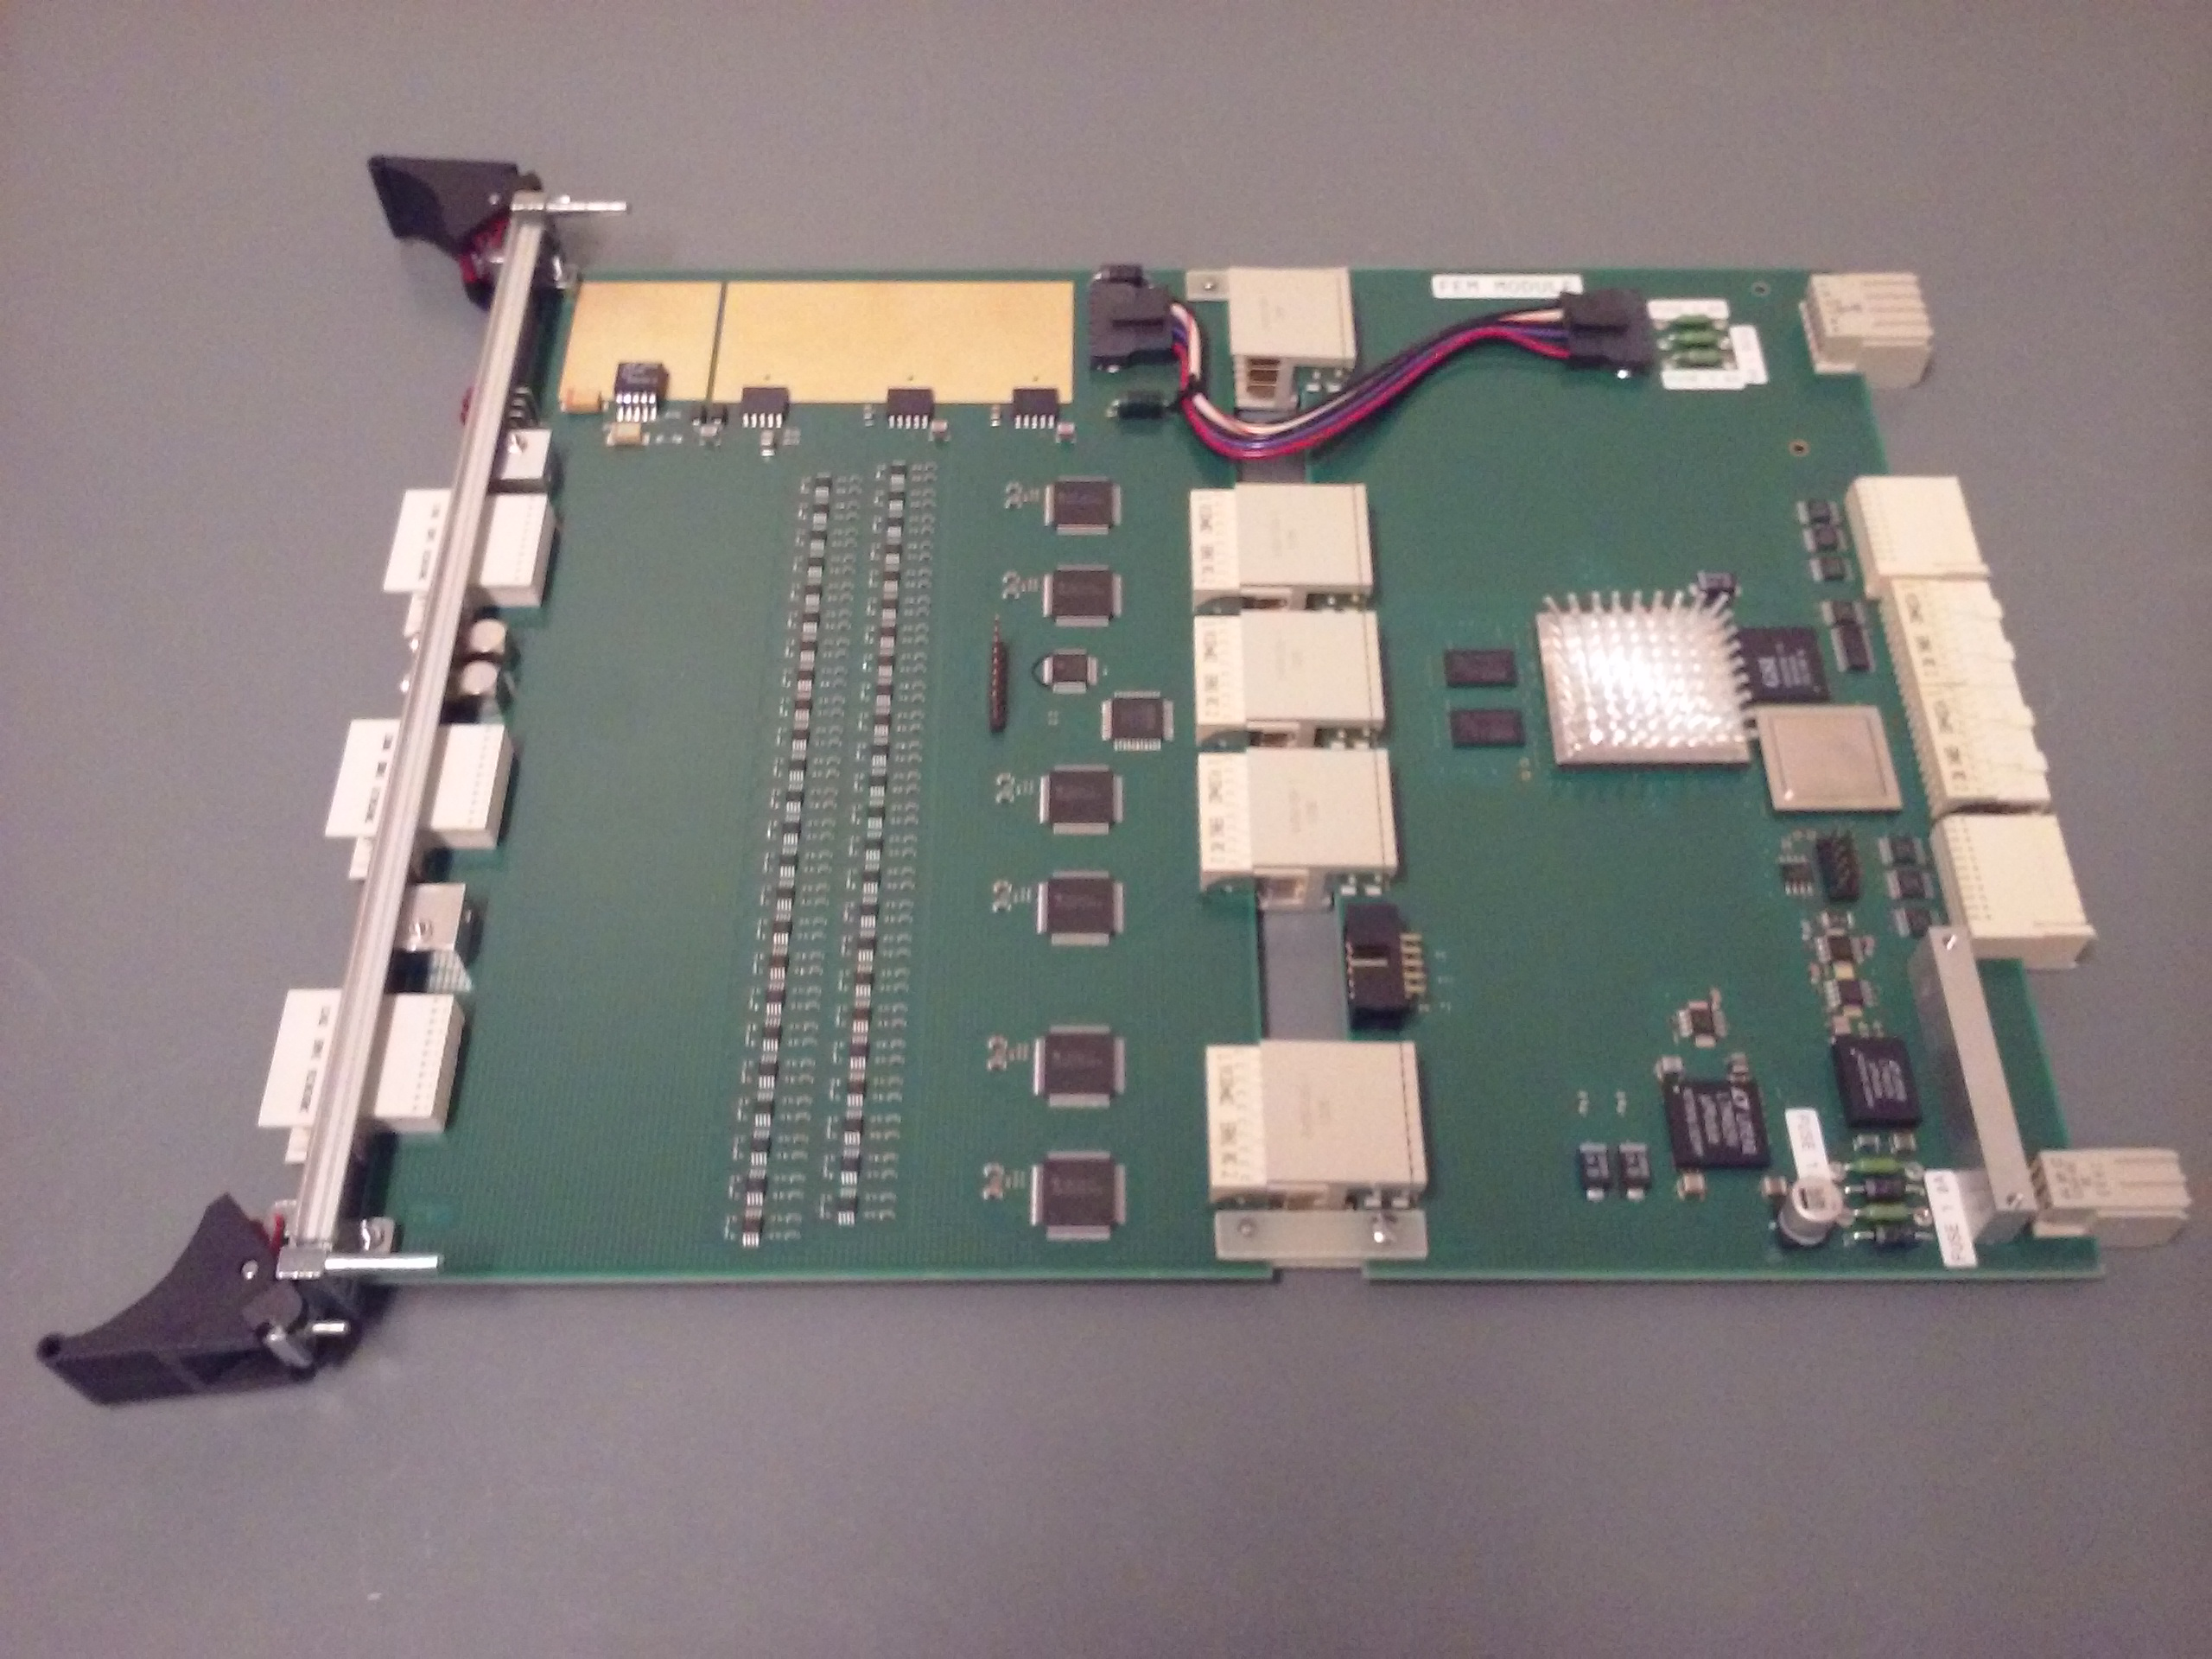
\includegraphics[width=0.8\linewidth]{./figures/PMTshaper.jpg}%
\caption{\label{fig:readout_8}The PMT readout board digitizes 48 input signals.}
\end{figure}

In addition to HG and LG waveforms from the PMTs, each readout board also receives, digitizes, and processes beam gate signal markers which arrive 4$\mu$s before the BNB 1.6$\mu$s and NuMI 10$\mu$s beam gates. These gates are used to (a) specially mark regions of interest where PMT data are read out continuously with no compression and (b) look for coincident PMT light signatures for trigger generation. 

\subsubsection{Data Handling and PMT Trigger Generation}
\label{tpcfem}

PMT information is recorded in the NU data stream for four 1.6 ms frames associated with an event trigger: the frame containing the (asynchronous) trigger, the frame preceding the trigger frame, and two frames following the trigger frame. To avoid the inordinate amount of data that would be generated at a 64 MHz sampling rate, the FEM applies a zero-suppression immediately after digitization, retaining only samples above a given threshold as well as enough information before and after this useful data to establish a local baseline value; this collection of information is referred to as a PMT readout ROI. An exception is formed for beam-related or other likewise-triggered data where, for example,  the 4$\mu$s-early BNB and NuMI beam gates mentioned in section~\ref{sec:pmtdigit} instruct readout of 1500 consecutive samples (23.4$\mu$s) surrounding and including the beam gates regardless of signal activity.

Two different discriminators are used: one that is active inside the beam gate(s), and one that is also active outside the beam-gate-surrounding 23.4$\mu$s. The latter discriminator governs the readout activity due to cosmic rays and other non-beam related activity. The first discriminator enables PMT channels with pulse heights above a configurable threshold (e.g. corresponding to 1 photoelectron)  to participate in trigger multiplicity and pulse height sum conditions, as described in the following section. The thresholds for those two discriminators are set to different levels and configured with different dead times for the HG and LG signals.

\subsection{Level-1 Trigger Generation}
\label{sec:trigger}

The TB, which physically resides in the PMT readout crate, issues a ``Level-1'' trigger in order to flag frames that must be treated differently. In the case of the \lartpc readout, the TB flags the 4 frames that must be trimmed and readout through the NU data stream and, in the case of the PMT readout, it flags the 4 frames that must be readout in full through the NU data stream.

The inputs to the TB include a BNB trigger input (maximum rate of 15 Hz), a NuMI trigger input (1.25 Hz), a Fake Beam trigger input (configurable), a PMT trigger input, and two calibration trigger inputs, provided by the laser calibration system and the cosmic ray muon telescope, respectively. The TB also has the ability to receive, via the crate controller, DAQ-issued calibration triggers, which are used explicitly for cold electronics and PMT calibration. The various input triggers can be independently pre-scaled, masked, and mixed together (OR or AND) to generate an event trigger.

The FPGA firmware in the PMT FEM can generate two different types of PMT triggers based on the PMT signals: a cosmic PMT trigger and a beam gate PMT trigger. Beam gate PMT triggers are configured in the same way for the BNB, NuMI, and Fake Beam. The nominal criteria for these triggers are (1) PMT multiplicity $\ge$1 and (2) summed PMT pulse-height $\ge$ 2 photoelectrons (p.e.) summed over all 32 HG1 PMT channels. Both criteria must be met during any 100 ns time interval coincident with the beam spill duration (1.6$\mu$s in the case of the BNB and Fake Beam gates and 10$\mu$s in the case of the NuMI gate), and only channels enabled by the beam gate discriminator can participate in the active pulse-height and multiplicity sums. The criteria for a cosmic PMT trigger are (1) PMT multiplicity $\ge$1 and (2) summed PMT pulse-height $\ge$ 40 p.e. summed over any one of 28 preset groups of 5 HG2 PMT channels that are grouped based on their spatial correlation. Again, only channels enabled by the cosmic discriminators can participate in the trigger generation.

In addition, a software-based algorithm has been written to mimic the capabilities of the beam gate PMT trigger performed in the FPGA and provide more flexibility in trigger criteria settings. Details of this higher-level software trigger are described in section~\ref{sec:software-trigger}.

%During normal running, the BNB and NuMI beam gates can be OR'd or put in coincidence with the PMT beam gate trigger in the TB. Since most of the BNB and NuMI beam gates are expected to yield no neutrino interactions, placing them in coincidence with the PMT beam gate triggers significantly enhances the neutrino interaction candidate purity in the BNB and NuMI data. 

Figure~\ref{fig:readout_9} diagrams the PMT readout and trigger logic. Activation or masking of each of the trigger inputs and outputs is DAQ-controlled. The trigger condition and explicit PMT trigger type, if applicable, is available for every event in the NU data stream at both the event-building stage and offline; this information is read out via a dedicated optical data stream, directly from the TB. The trigger number and trigger time are also propagated and available in the NU data streams arriving independently at the assembler DAQ machine from each \lartpc and PMT crate, and can therefore be used to correctly associate data from the same event.

\begin{figure}
\centering
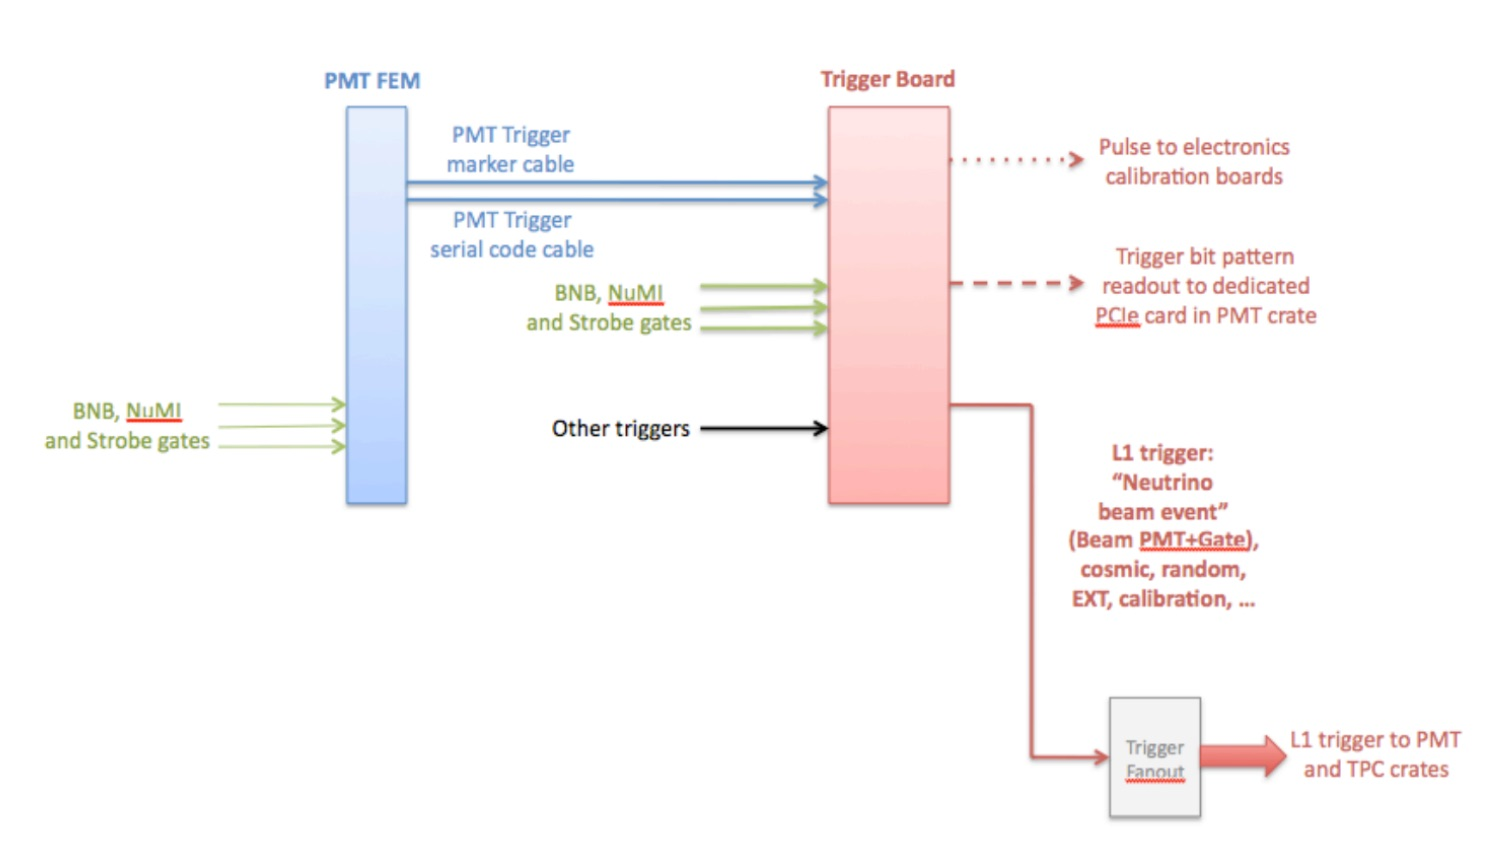
\includegraphics[width=0.8\linewidth]{./figures/readout_9.jpg}%
\caption{\label{fig:readout_9}PMT readout and trigger logic.}
\end{figure}

The readout control sequence is illustrated in figure~\ref{fig:readout_10}. When a trigger is generated by the TB it is passed to a fan-out module on a single cable and from there it is distributed to all crate controllers (\lartpc and PMT). Through the crate backplane, the trigger gets propagated to each FEM. An FEM that receives a trigger temporarily inhibits the SN stream with its associated decimation and initiates the loss-less readout scheme to direct the data to the appropriate readout path. SN readout resumes once the XMIT is done sending all NU data associated with an event to the DAQ. 

\begin{figure}
\centering
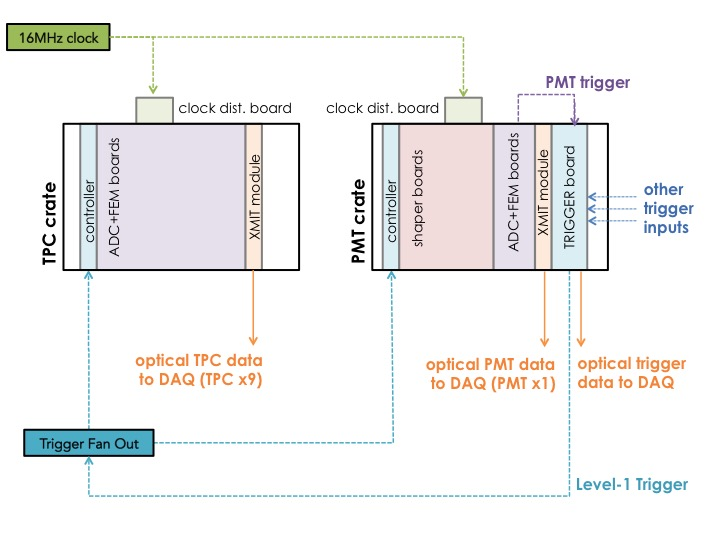
\includegraphics[width=0.8\linewidth]{./figures/det_figure_10.jpg}%
\caption{\label{fig:readout_10}Readout control sequence. The MicroBooNE Level-1 trigger is a hardware trigger which consists of the OR between a BNB, NuMI, and EXT (strobe) trigger. Once received, the Level-1 trigger is propagated to all readout crates and instructs PMT and TPC data readout into ten dedicated sub-event buffer DAQ machines. The data across different DAQ machines is correlated at event building stage by the trigger number and corresponding trigger frame and sample numbers recorded in each data stream, per event. All readout crates are synchronized and correlated to the same 16 MHz clock.}
\end{figure}

%************************************
% DAQ
%\input{daq}
\subsection{DAQ Design}
\label{sec:daq}
%Eric Church - Aug. 2015
The MicroBooNE DAQ system acquires data from the readout electronics, writes data to local disk before transferring it to long-term storage, configures and controls the readout electronics during data-taking periods, and monitors the data flow and detector conditions. These tasks are performed on a network of commodity servers running both custom and open-source software.

The data from each crate of the backend electronics is sent to a dedicated server (called the sub-event buffer, or SEB) via an optical fiber, arriving in a card on the SEB's PCIe bus. A real-time application places these data in an internal buffer, collects all segments belonging to an event, and creates a sub-event fragment that may be routed to a specified destination.  For the NU stream, in which the data arrives with every trigger, these fragments are sent to a single event-building machine (EVB) over an internal network. Full events are checked for consistency and written to local disk on the EVB before being sent offline for further processing. A high-level software trigger, described in section~\ref{sec:software-trigger}, is applied to the data to determine whether events should be written locally or ignored. For the SN stream the data remains on the SEB where it is written to disk and only sent for offline analysis on explicit requests.

Data writing to either triggered or SN streams is limited by the RAID6 disk write speeds which are roughly 300 MB/sec. This is much less than the network bandwidth bottleneck, which is 10 Gbps. The 300 MB/sec disk write speed therefore sets the maximum aggregate rate at which all SEB fragments can ship data to the EVB without loss of data. With Huffman compression, which gives a data reduction of approximately a factor of five (figure~\ref{fig:readout_6}) and the PMT trigger, which reduces the data rates by another factor of $>70$, this is more than sufficient for MicroBooNE's maximum 15 Hz beam spill rate. MicroBooNE expects a total triggered write rate of around 12 MB/sec. The SN stream circular buffers, which will be aggressively (non-losslessly) compressed beyond what the triggered stream experiences, will fill each server's 14 TB in on the order of one day, which is ample time to respond to a Super Nova Early Warning System (SNEWS) alert \cite{Scholberg:2008fa}.

After data is written to disk, it is then copied to another server on the internal DAQ network, where the raw data is further compressed, shipped, and queued to be stored on in tape and disk cache using the Fermilab central data management system known as SAM.  Offline applications then begin processing the raw data, converting the binary data format into a LArSoft \cite{larsoft} ROOT-based format which can be used as input for reconstruction algorithms.  LArSoft is a common framework of software tools utilized by many \lartpc experiments at Fermilab and elsewhere.  A separate process collects beam data and, during binary to LArSoft conversion, inserts that data into the built events. A duplicate copy of the data is also stored offsite at Pacific Northwest National Laboratory (PNNL). This collection of approximately 15 ``projects''  and the database which holds and monitors the state of the data flow is known as the Python/Postgres for MicroBooNE Scripting system (PUBS), and is patterned after a similar database state machine that the Double Chooz experiment used for data management.  As PUBS pushes the data through this process, the progress of each project is monitored and viewable via GUI. PUBS can also monitor the state of the SN stream data, held locally on the SEBs.  A separate offline PUBS instance controls the processing of the data, including applying newly calculated calibration constants as part of data quality management.  Figure \ref{fig:dataflow} schematically depicts the flow of data throughout the MicroBooNE DAQ system.

\begin{figure}
\centering
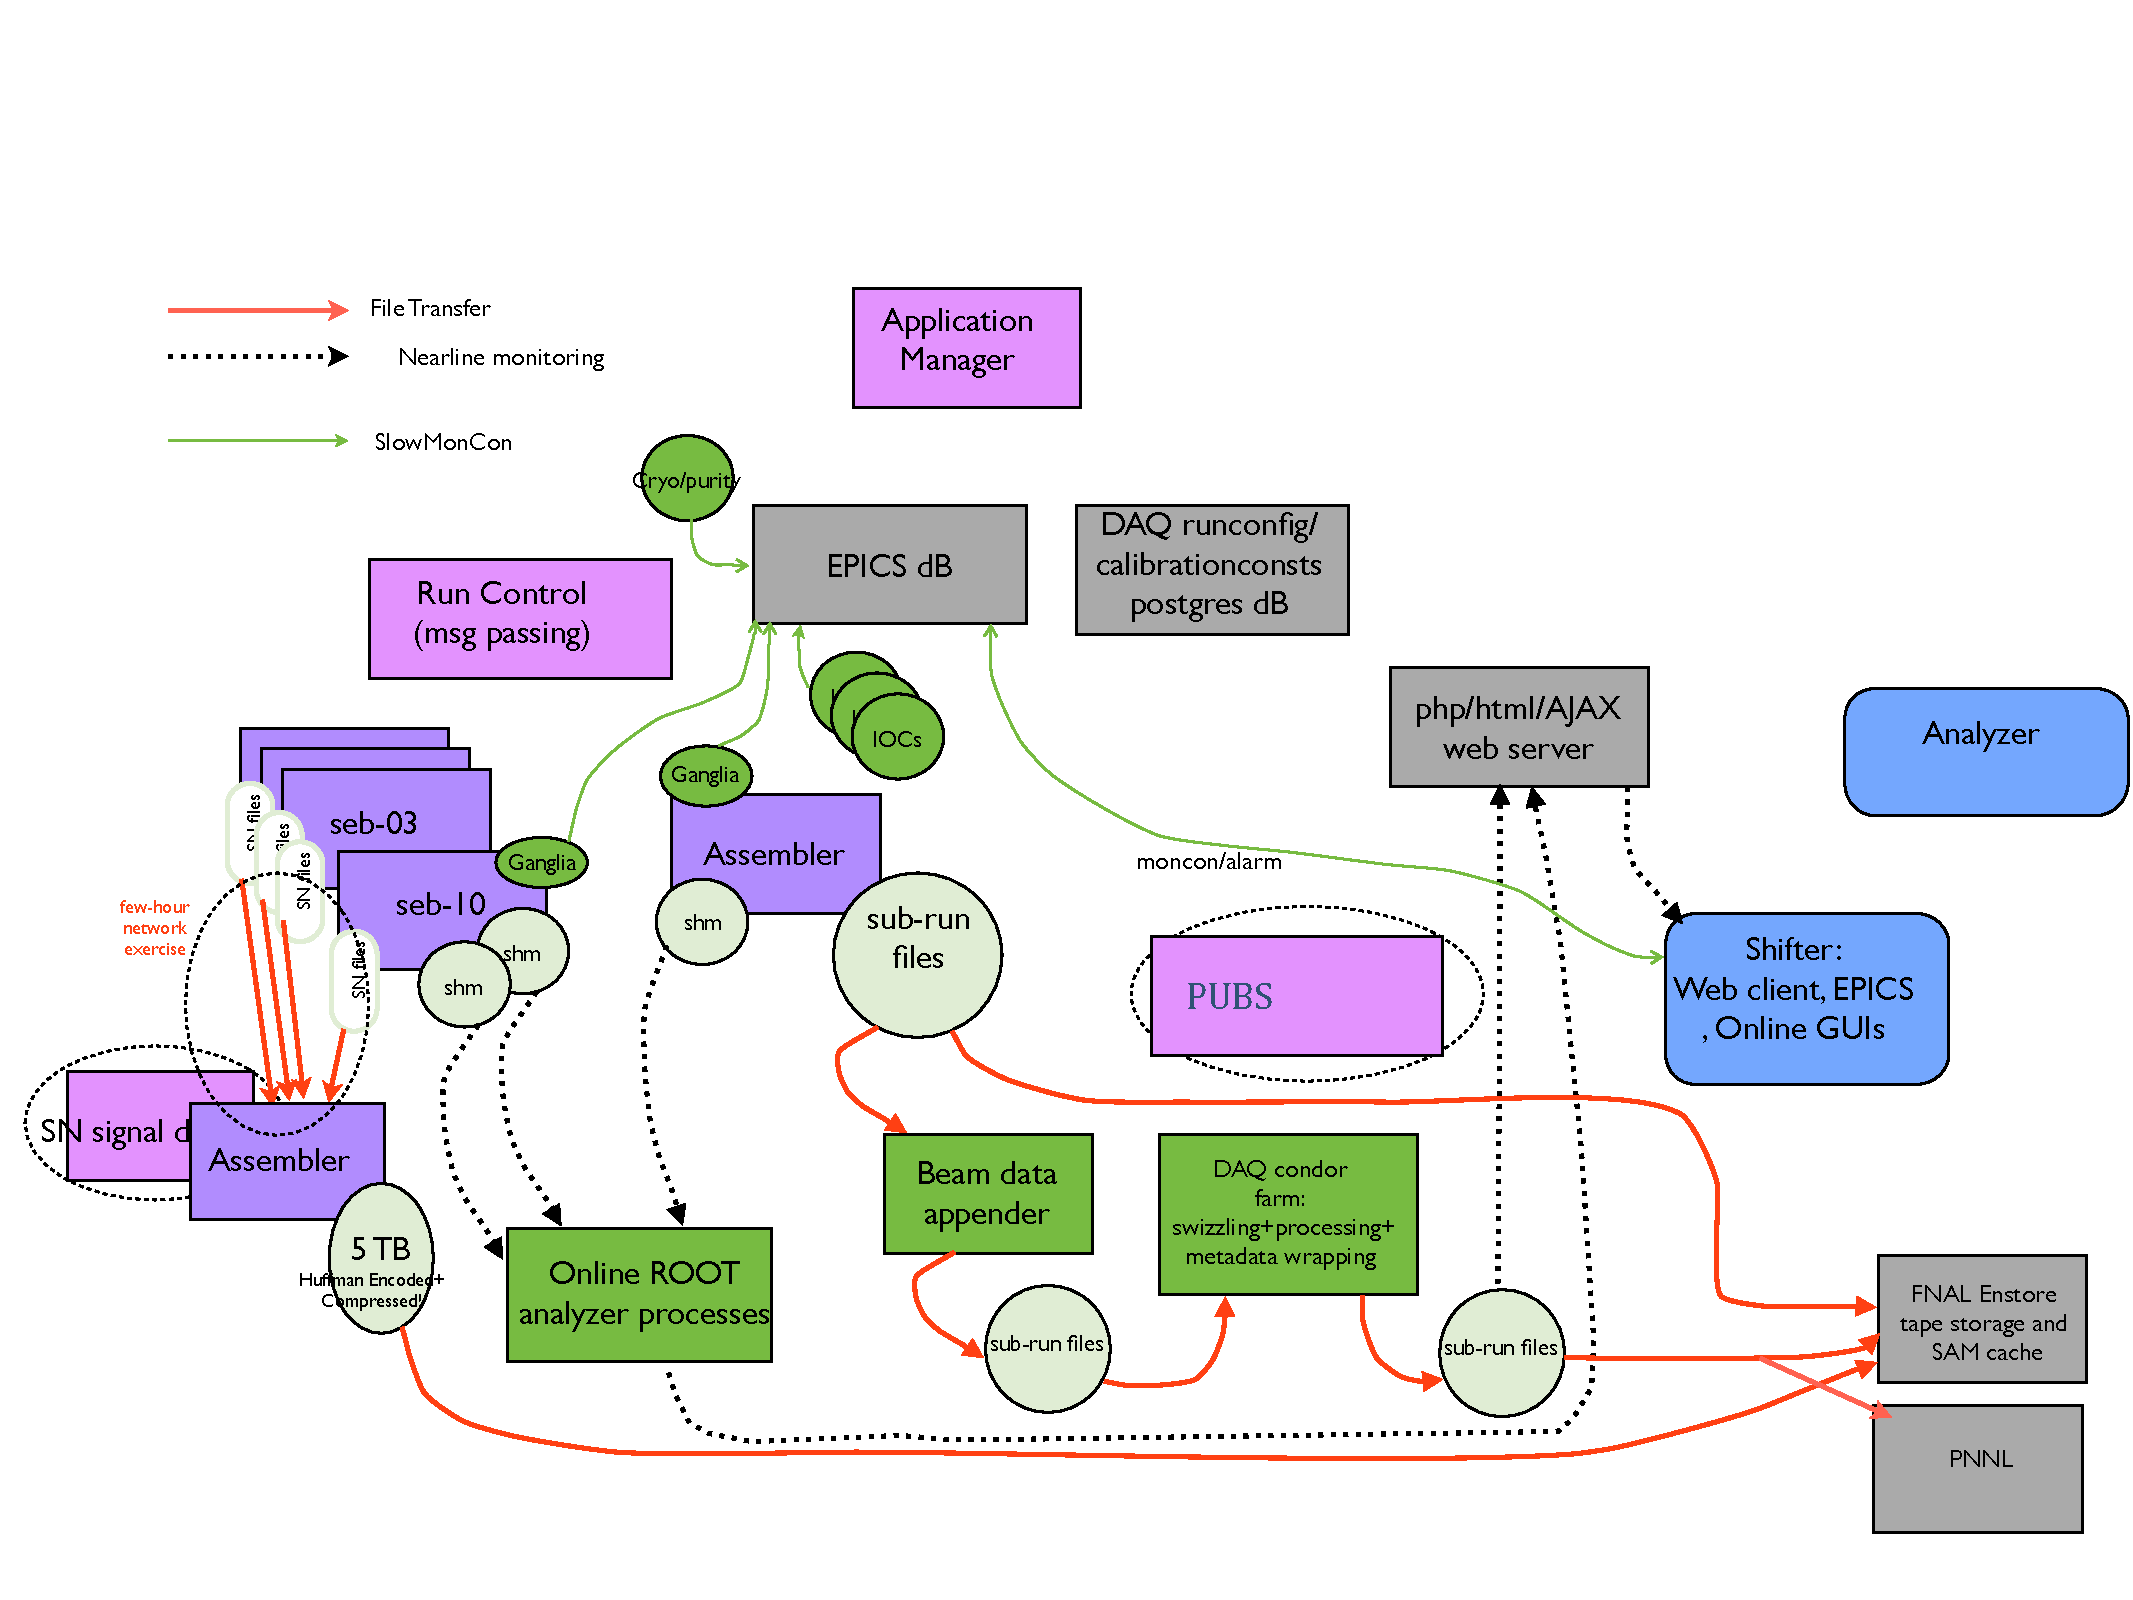
\includegraphics[width=0.95\textwidth]{./figures/dataFlow.pdf}
\caption{Data flow for MicroBooNE DAQ from raw to processed.}
\label{fig:dataflow}
\end{figure}


Additional software components handle the management of the main DAQ processes moving the data. A run control application issues configuration and state-progressing commands to the SEBs and EVB. Configuration states are stored in a dedicated run configuration database, which allows for the setting and preserving of configuration information for the DAQ, readout, and additional components. This database not only allows for creating the large ($\sim$200 parameters) intricate DAQ run configuration files, but also enforces certain conditions which must hold for consistency. For example, the configuration that initiates the ASICS charge-injection calibration also dials and captures the settings on the external pulser that drives the calibration signal and assures that ASICS gains and peaking time parameters are enforced and recorded. %The configuration that runs the PMT flasher calibration additionally ensures that the charge-injection is only run simultaneously, if desired, in certain allowed modes. 

Another important aspect of the system is monitoring the health of the DAQ. Monitoring of DAQ components is accomplished through Ganglia which monitors basic system states (such as CPU, memory, and network usage) as well as allows use of custom metrics to monitor the data flow and status of the readout electronics \cite{GangliaBook}. These metrics are sampled and collected by the EPICS slow monitoring and control processes, which archives desired quantities and provides alarms when pre-defined thresholds are exceeded \cite{EPICS}. Some examples of Ganglia metrics that are monitored and alarmed in EPICS are the rates of growth of the SEB data buffers, the fragment rates leaving each SEB, and fragment arrival rates at the EVB.  Figure \ref{fig:ganglia} shows examples of Ganglia metrics.  

\begin{figure}
\centering
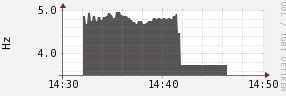
\includegraphics[width=0.45\textwidth]{./figures/ganglia_EXT_trigRate.png}
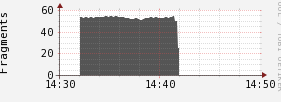
\includegraphics[width=0.45\textwidth]{./figures/ganglia_RECEIVEDfrag_rate.png}\\
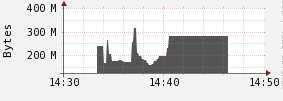
\includegraphics[width=0.45\textwidth]{./figures/ganglia_WRITEdata_rate.png}
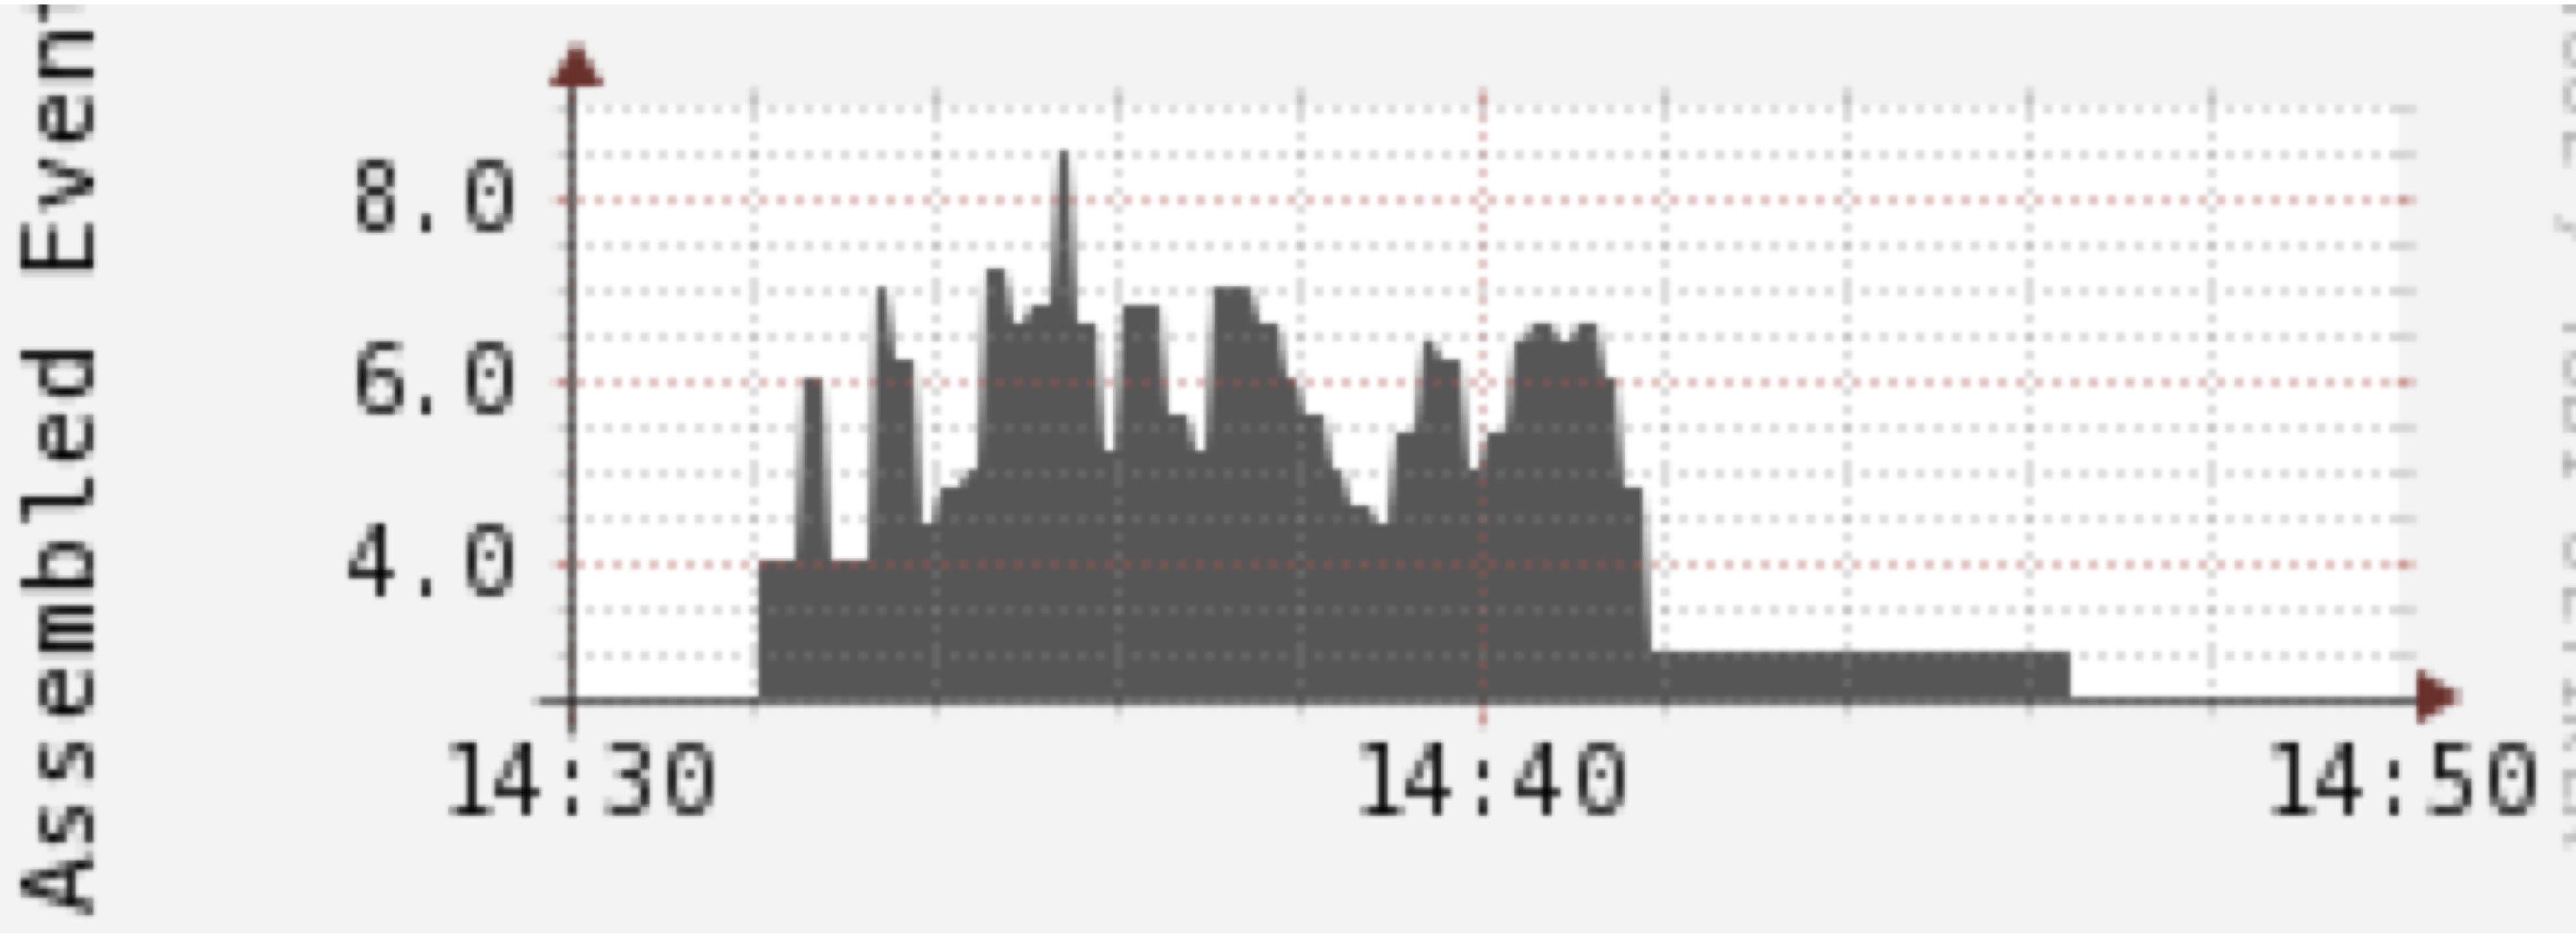
\includegraphics[width=0.45\textwidth]{./figures/ganglia_WRITEQUE_size.png}
%\caption{Ganglia metrics showing data flow on the EVB machine during a 2 Hz test run. (ul) the event disk write rate (ur) The number of assembled queued-up events waiting to be written (ll) The total EVB received data rate, and the (lr) received fragment rate.}
\caption{Ganglia metrics showing data flow on the EVB machine during a 5 Hz test run. Shown are the external trigger rate (top-left), the received fragment rate (top-right), the disk data write rate (bottom-left), and the number of assembled queued-up events waiting to be written (bottom-right). (11 fragments constitute a complete event in the MicroBooNE DAQ.)}
\label{fig:ganglia}
\end{figure}

Additional online monitoring exists to check data quality in more detail, through both programmed checks and visual checks including a real-time event display. The online monitoring takes snapshots into shared memory segments on the SEBs and the EVB, and thus provides the desired low latency checks of newly-arriving data. It continually walks through these $\approx 150$ MB snap-shotted events and outputs histograms of occupancies and rates which are saved in ROOT files \cite{BRUN199781}. The histograms are then displayed in a web-based monitoring system that is easily accessible by the shift crew. Channels are aggregated in a variety of formats, including the order in which they appear in crates or across the wires and PMTs themselves. In this way, potential problems across connectors or crates, for example, may be more readily identified. Noisy, quiet, and unresponsive channels are easily marked and displayed to the shift crew.  Figure \ref{fig:onlinemonitor} shows an example of available online monitoring information.

\begin{figure}
\centering
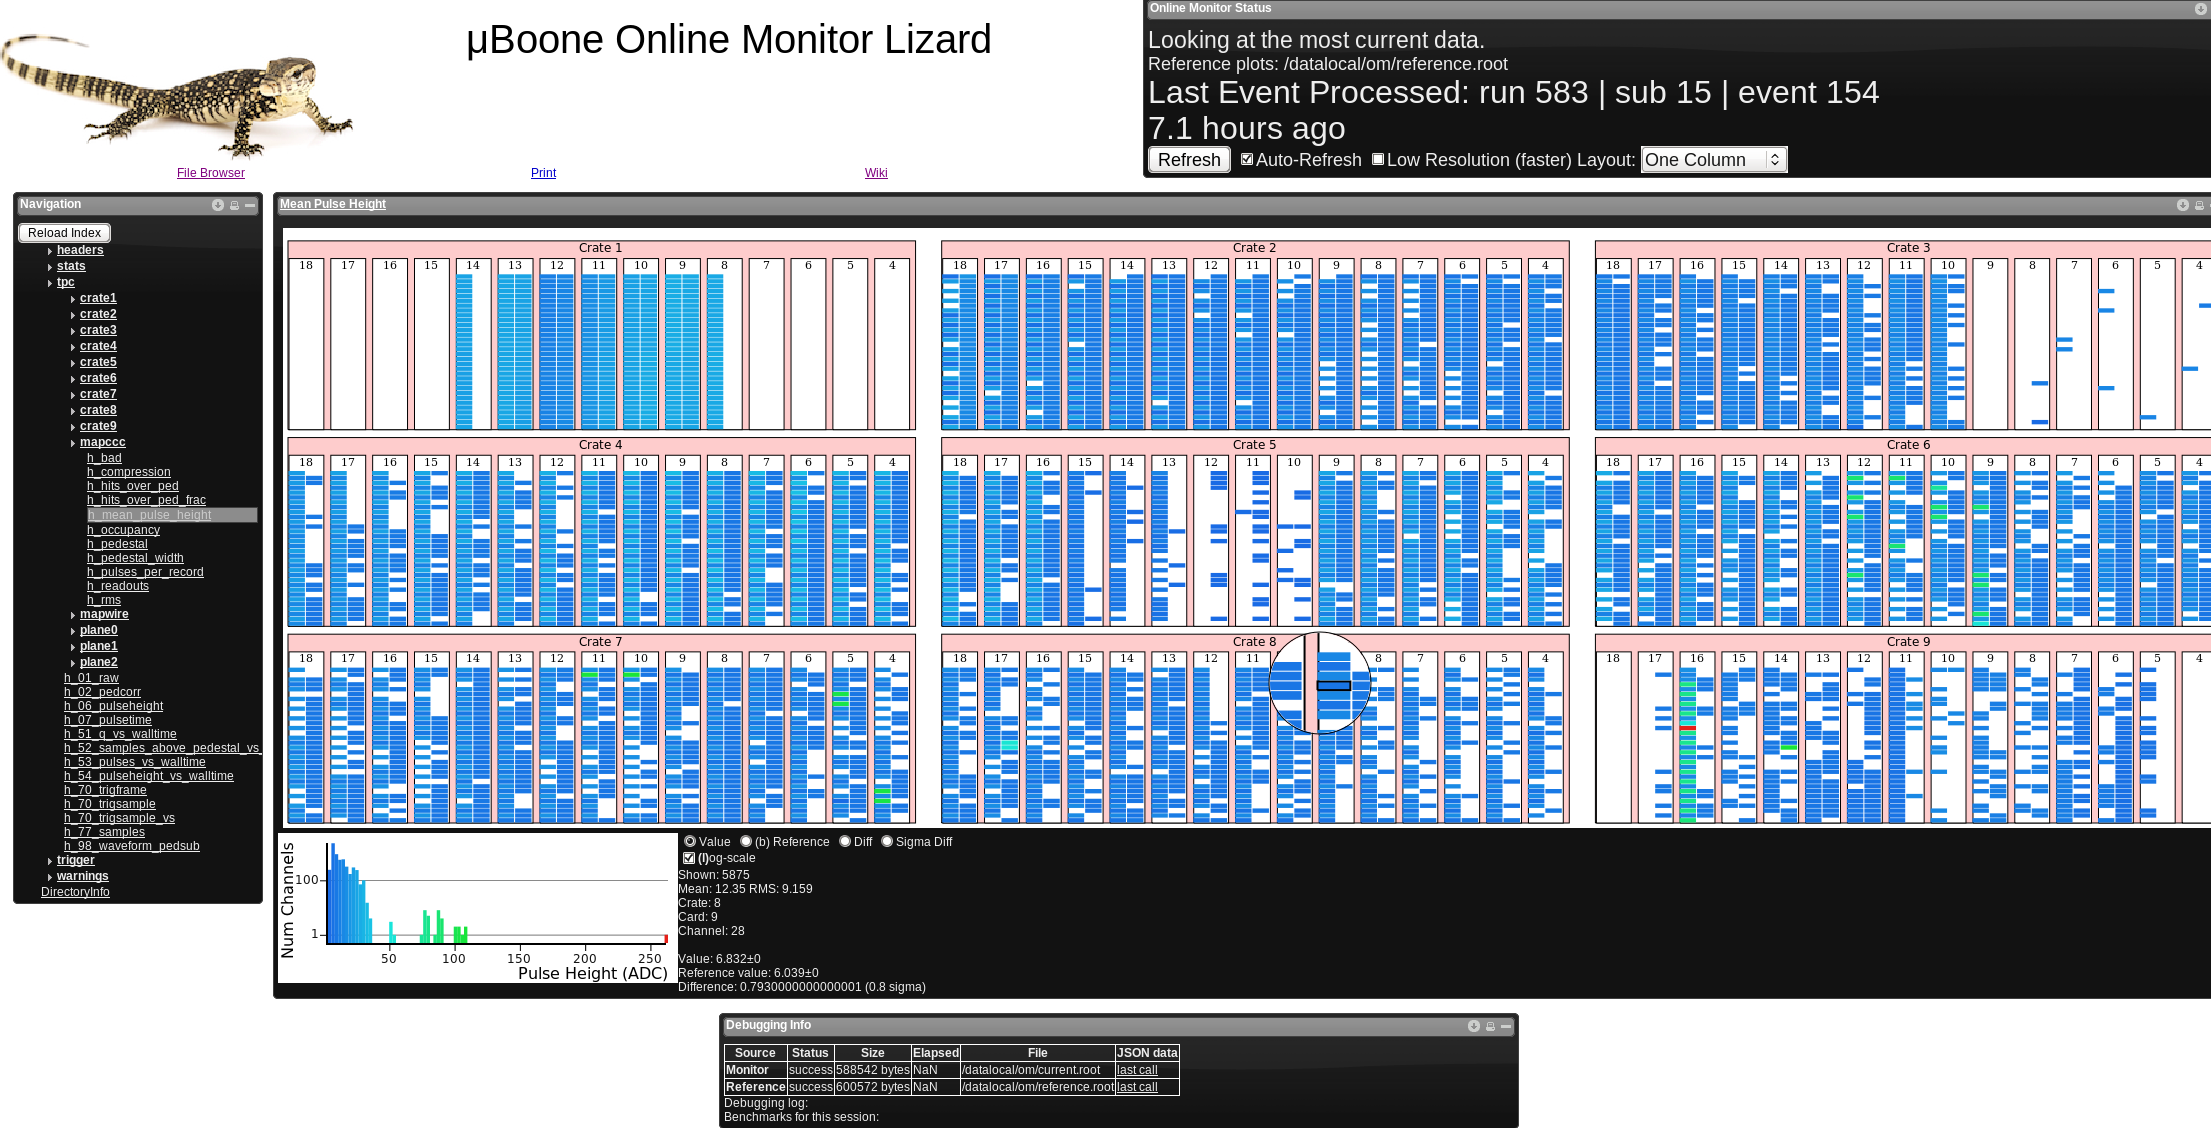
\includegraphics[width=0.95\textwidth]{./figures/daqLizard.png}
\caption{The online monitoring GUI (Lizard). The pedestal-subtracted ADC values for all 8256 wires in one minimum bias event are shown. Each box is a channel. Not all crates are fully populated with electronics. }
\label{fig:onlinemonitor}
\end{figure}

\subsection{High-level software trigger}
\label{sec:software-trigger}
After events are collected on the DAQ event-builder server, a suite of trigger algorithms are applied to the data. Currently, these algorithms mimic the PMT readout electronics' FPGA-based beam gate trigger algorithms, described in section~\ref{sec:trigger}. A search over the PMT digitized waveforms from the beam-spill period is performed, and if there is a significant amount of light in coincidence with the expected arrival time of the neutrinos, the event is marked and saved. This selection is performed on data that passes the level-1 trigger, which typically includes data from the BNB and NuMI beams, and randomly selected off-beam data from an ``external'' trigger. A fraction of the data from each of these level-1 trigger input streams is also retained via a random prescale, which provides a selection of data that has not been biased by the trigger. The high-level trigger algorithms take approximately 10 ms to return a result, a latency that is well-below the event-taking rate and so does not impact data-taking performance. The average pass rate for data-events in the PMT beam gate trigger algorithm is roughly 5\%. 

%Note from Mitch - commenting out following "slow mon" description since it also is provided in the "slow-controls.tex" writeup in a bit more detail.

%For slow controls, MicroBooNE uses EPICS, an Argonne National Labs open source slow monitoring and control system used widely in the nuclear and high energy physics communities. EPICS monitors and catalogues many types of detector data at sample rates on the order of 1 Hz. This data spans computer server health metrics -- including gathering Ganglia's measured fan speeds, temperatures, RAID health metrics -- to cryogenics and argon purity, to drift and wire bias high voltages, electronics voltages, beam data latency, etc. A series of single board computers or ``Glomations'' residing in electronics racks connect to RTDs that measure ambient temperatures and rack fan speeds and provide the interface to the EPICS database that runs on one of the DAQ servers.  Figure \ref{fig:slowmon} shows an example of slow monitoring data recorded during a portion of MicroBooNE's initial liquid argon filling.  The Glomations also provide the control interface to the drift and PMT high voltages. Meanwhile the EPICS GUI provides the interface to the 10 ``crate rails'' power supplies as well as to all of the cold ASICS power via locally switched ethernet.
%
%\begin{figure}
%\centering
%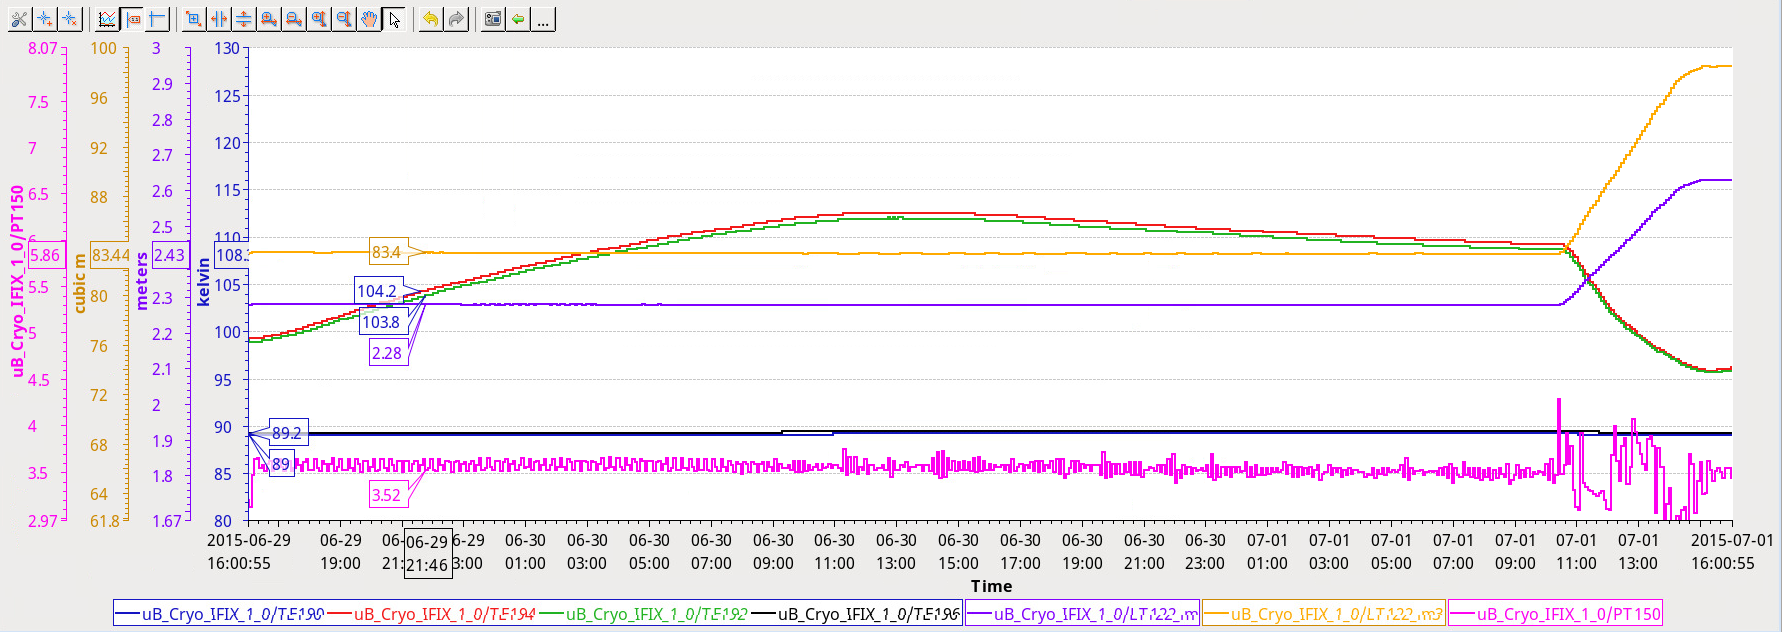
\includegraphics[width=0.95\textwidth]{./figures/fill_01-July-2015.png}
%\caption{Slow monitoring data of liquid argon fill levels and temperatures spanning two separate fills over two days in MicroBooNE. Shown are the fill level and volumes along with two temperatures on two RTDs along the top \lartpc frame}
%\label{fig:slowmon}
%\end{figure}





